\makeatletter \@ifundefined{rootpath}{% Manual to memoir http://mirrors.dotsrc.org/ctan/macros/latex/contrib/memoir/memman.pdf

%\documentclass[a4paper,12pt,fleqn,openany,twoside]{memoir} %two sides for printing
\documentclass[a4paper,12pt,fleqn,openany,oneside]{memoir} %one side for pdf
\usepackage[english]{babel}
\usepackage[utf8]{inputenc}
\usepackage{microtype}
\usepackage{paralist}

%Definitions
\usepackage{amsthm}
\theoremstyle{plain}
\newtheorem{thm}{Theorem}[chapter] % reset theorem numbering for each chapter
\theoremstyle{definition}
\newtheorem{defn}[thm]{Definition}

% Choses the depth of numerations
\setsecnumdepth{subsubsection}

% Choses the depth of toc
%\maxtocdepth{subsection}

% Turn figures sideways with \begin{sideways} figure \end{sideways}
\usepackage{rotating}

% LaTeX logical statements
\usepackage{ifthen}

% Fancy space after use of e.g. command
\usepackage{xspace}

% Skips after paragraphs
\usepackage{parskip}

% Layout settings
\setlength{\parindent}{0cm}
\setlength{\parskip}{2ex plus 2ex} %kan udvides til f.eks: '2ex plus 2ex minus 0ex'

\sloppybottom

% Don't make a collection per default
\newcommand{\worksheetcollection}{false}

% Bibtex
\usepackage[square,numbers,sort,comma]{natbib}
%\usepackage{cite}
%\bibliographystyle{plainnat}
\bibliographystyle{IEEEtran}


% Fixmes
\usepackage{fixme}
\fxsetup{draft}

% Mathematic
\usepackage{amsmath}
\usepackage{amsfonts}
\usepackage{amssymb}
\usepackage{stmaryrd}
\allowdisplaybreaks[1]


% Acronyms
\usepackage[printonlyused]{acronym}

% Images
\usepackage{graphicx}
\usepackage{wrapfig}
\usepackage[outdir=./]{epstopdf}
\usepackage{epsfig}


% Captions ans subcaptions
\captionnamefont{\footnotesize\bfseries}
\captiontitlefont{\footnotesize}

% Enable memoir subfloats for figures and tables
\newsubfloat{figure}
\newsubfloat{table}

% Hack memoir subfigure styles to have bold label and footnotesize fonts
\renewcommand{\thesubfigure}{\footnotesize\bfseries{(\alph{subfigure})}}
\renewcommand{\thesubtable}{\footnotesize\bfseries{(\alph{subtable})}}

\renewcommand{\subcaption}[2][]{\subbottom[\footnotesize{#1}]{#2}}

% Memoir tweak pagenumbers
%\pagestyle{headings}

% Tikz
\usepackage{tikz}
\usetikzlibrary{arrows,shapes,calc,positioning}
\pgfmathsetseed{1}

%Pgf plots
\usepackage{pgfplots}
\pgfplotsset{compat=1.5}
% loatbarrier, keep figures within (sub,subsub) sections
\usepackage{placeins}
\usepackage{pgfplots}
\usepgfplotslibrary{units}
\usepackage[space-before-unit,range-units = repeat]{siunitx}

% Hyperlinked auto references
\usepackage[hidelinks]{hyperref}
\usepackage[nameinlink]{cleveref}
\crefname{lstlisting}{Listing}{Listings}  
\Crefname{lstlisting}{Listing}{Listings}

\crefname{thm}{definition}{definitions}
\Crefname{thm}{Definition}{Definitions}

%\def\chapterautorefname{Kapitel}
%\def\sectionautorefname{Afsnit}
%\def\subsectionautorefname{Afsnit}
%\def\subsubsectionautorefname{Underafsnit}
%\def\figureautorefname{Figur}
%\def\lstlistingautorefname{Listing}
%\def\lstnumberautorefname{Linje}
%\def\itemautorefname{Punkt}
\usepackage[hypcap]{caption} % Link to top of the figure and not the caption

%Sick shit to make \Autoref command
%http://tex.stackexchange.com/questions/36575/autorefs-inserted-text-has-not-the-correct-case
\def\HyLang@english{%
  \def\equationautorefname{Equation}%
  \def\footnoteautorefname{Footnote}%
  \def\itemautorefname{item}%
  \def\figureautorefname{Figure}%
  \def\tableautorefname{Table}%
  \def\partautorefname{Part}%
  \def\appendixautorefname{Appendix}%
  \def\chapterautorefname{Chapter}%
  \def\sectionautorefname{Section}%
  \def\subsectionautorefname{Subsection}%
  \def\subsubsectionautorefname{Subsubsection}%
  \def\paragraphautorefname{Paragraph}%
  \def\subparagraphautorefname{Subparagraph}%
  \def\FancyVerbLineautorefname{Line}%
  \def\theoremautorefname{Theorem}%
  \def\pageautorefname{Page}%
}

% Reference greencommentssections with number and name
\usepackage{nameref}
\newcommand{\bsnameref}[1]{\Cref{#1} ``\nameref{#1}''}
\newcommand{\bsref}[1]{\Cref{#1}}
\newcommand{\bsbilagref}[1]{Appendix \ref{#1}}
\newcommand{\bsbilagnameref}[1]{Appendix \ref{#1} ``\nameref{#1}''}
\newcommand{\pling}[1]{``#1''}


% Listings for code qoutes
\usepackage{listings}
%\usepackage[usenames,dvipsnames,svgnames,table]{xcolor}
\usepackage{color}
\usepackage{xcolor}
\definecolor{bluekeywords}{rgb}{0.13,0.13,1}
\definecolor{greencomments}{rgb}{0,0.5,0}
\definecolor{redstrings}{rgb}{0.9,0,0}
\usepackage{caption} 
\usepackage{multicol}
\DeclareCaptionFont{white}{\color{white}}
\DeclareCaptionFormat{listing}{\colorbox{gray}{\parbox{\textwidth}{#1#2#3}}}
\captionsetup[lstlisting]{format=listing,labelfont=white,textfont=white}
%\lstset{numbers=left}
\usepackage{courier}
\lstset{
	basicstyle=\footnotesize\ttfamily,
	tabsize=2,
	breaklines=true,
  literate={æ}{{\ae}}1 {ø}{{\o}}1 {å}{{\aa}}1 {Æ}{{\AE}}1 {Ø}{{\O}}1 {Å}{{\AA}}1,
  keywords={typeof, new, true, false, catch, function, return, null, catch, switch, var, if, in, while, do, else, case, break},
  keywordstyle=\color{blue}\bfseries,
  ndkeywords={class, export, boolean, throw, implements, import, using, this},
  ndkeywordstyle=\color{darkgray}\bfseries,
  identifierstyle=\color{black},
  sensitive=false,
  comment=[l]{//},
  morecomment=[s]{/*}{*/},
  commentstyle=\color{purple}\ttfamily,
  stringstyle=\color{red}\ttfamily,
  numbers=left,
  numbersep=-5pt,
  showstringspaces=false,
  showspaces=false,
  %morestring=[b]',
  %morestring=[b]"
}
\lstnewenvironment{code}[1][]%
  {\minipage{\linewidth} 
   \lstset{basicstyle=\ttfamily\footnotesize,frame=single,#1}}
  {\endminipage}

\lstdefinelanguage{scala}{
  morekeywords={abstract,case,catch,class,def,%
    do,else,extends,false,final,finally,%
    for,if,implicit,import,match,mixin,%
    new,null,object,override,package,%
    private,protected,requires,return,sealed,%
    super,this,throw,trait,true,try,%
    type,val,var,while,with,yield, Unit, Boolean, Int},
  otherkeywords={=>,<-,<\%,<:,>:,\#,@},
  sensitive=true,
  morecomment=[l]{//},
  morecomment=[n]{/*}{*/},
  morestring=[b]",
  morestring=[b]',
  morestring=[b]"""
}

\lstdefinelanguage{clojure}%
{morekeywords={*,*1,*2,*3,*agent*,*allow-unresolved-vars*,*assert*,*clojure-version*,*command-line-args*,%
*compile-files*,*compile-path*,*e,*err*,*file*,*flush-on-newline*,*in*,*macro-meta*,%
*math-context*,*ns*,*out*,*print-dup*,*print-length*,*print-level*,*print-meta*,*print-readably*,%
*read-eval*,*source-path*,*use-context-classloader*,*warn-on-reflection*,+,-,->,->>,..,/,:else,%
<,<=,=,==,>,>=,@,accessor,aclone,add-classpath,add-watch,agent,agent-errors,aget,alength,alias,%
all-ns,alter,alter-meta!,alter-var-root,amap,ancestors,and,apply,areduce,array-map,aset,%
aset-boolean,aset-byte,aset-char,aset-double,aset-float,aset-int,aset-long,aset-short,assert,%
assoc,assoc!,assoc-in,associative?,atom,await,await-for,await1,bases,bean,bigdec,bigint,binding,%
bit-and,bit-and-not,bit-clear,bit-flip,bit-not,bit-or,bit-set,bit-shift-left,bit-shift-right,%
bit-test,bit-xor,boolean,boolean-array,booleans,bound-fn,bound-fn*,butlast,byte,byte-array,%
bytes,cast,char,char-array,char-escape-string,char-name-string,char?,chars,chunk,chunk-append,%
chunk-buffer,chunk-cons,chunk-first,chunk-next,chunk-rest,chunked-seq?,class,class?,%
clear-agent-errors,clojure-version,coll?,comment,commute,comp,comparator,compare,compare-and-set!,%
compile,complement,concat,cond,condp,conj,conj!,cons,constantly,construct-proxy,contains?,count,%
counted?,create-ns,create-struct,cycle,dec,decimal?,declare,def,definline,defmacro,defmethod,%
defmulti,defn,defn-,defonce,defprotocol,defstruct,deftype,delay,delay?,deliver,deref,derive,%
descendants,destructure,disj,disj!,dissoc,dissoc!,distinct,distinct?,do,do-template,doall,doc,%
dorun,doseq,dosync,dotimes,doto,double,double-array,doubles,drop,drop-last,drop-while,empty,empty?,%
ensure,enumeration-seq,eval,even?,every?,false,false?,ffirst,file-seq,filter,finally,find,find-doc,%
find-ns,find-var,first,float,float-array,float?,floats,flush,fn,fn?,fnext,for,force,format,future,%
future-call,future-cancel,future-cancelled?,future-done?,future?,gen-class,gen-interface,gensym,%
get,get-in,get-method,get-proxy-class,get-thread-bindings,get-validator,hash,hash-map,hash-set,%
identical?,identity,if,if-let,if-not,ifn?,import,in-ns,inc,init-proxy,instance?,int,int-array,%
integer?,interleave,intern,interpose,into,into-array,ints,io!,isa?,iterate,iterator-seq,juxt,%
key,keys,keyword,keyword?,last,lazy-cat,lazy-seq,let,letfn,line-seq,list,list*,list?,load,load-file,%
load-reader,load-string,loaded-libs,locking,long,long-array,longs,loop,macroexpand,macroexpand-1,%
make-array,make-hierarchy,map,map?,mapcat,max,max-key,memfn,memoize,merge,merge-with,meta,%
method-sig,methods,min,min-key,mod,monitor-enter,monitor-exit,name,namespace,neg?,new,newline,%
next,nfirst,nil,nil?,nnext,not,not-any?,not-empty,not-every?,not=,ns,ns-aliases,ns-imports,%
ns-interns,ns-map,ns-name,ns-publics,ns-refers,ns-resolve,ns-unalias,ns-unmap,nth,nthnext,num,%
number?,odd?,or,parents,partial,partition,pcalls,peek,persistent!,pmap,pop,pop!,pop-thread-bindings,%
pos?,pr,pr-str,prefer-method,prefers,primitives-classnames,print,print-ctor,print-doc,print-dup,%
print-method,print-namespace-doc,print-simple,print-special-doc,print-str,printf,println,println-str,%
prn,prn-str,promise,proxy,proxy-call-with-super,proxy-mappings,proxy-name,proxy-super,%
push-thread-bindings,pvalues,quot,rand,rand-int,range,ratio?,rational?,rationalize,re-find,%
re-groups,re-matcher,re-matches,re-pattern,re-seq,read,read-line,read-string,recur,reduce,ref,%
ref-history-count,ref-max-history,ref-min-history,ref-set,refer,refer-clojure,reify,%
release-pending-sends,rem,remove,remove-method,remove-ns,remove-watch,repeat,repeatedly,%
replace,replicate,require,reset!,reset-meta!,resolve,rest,resultset-seq,reverse,reversible?,%
rseq,rsubseq,second,select-keys,send,send-off,seq,seq?,seque,sequence,sequential?,set,set!,%
set-validator!,set?,short,short-array,shorts,shutdown-agents,slurp,some,sort,sort-by,sorted-map,%
sorted-map-by,sorted-set,sorted-set-by,sorted?,special-form-anchor,special-symbol?,split-at,%
split-with,str,stream?,string?,struct,struct-map,subs,subseq,subvec,supers,swap!,symbol,symbol?,%
sync,syntax-symbol-anchor,take,take-last,take-nth,take-while,test,the-ns,throw,time,to-array,%
to-array-2d,trampoline,transient,tree-seq,true,true?,try,type,unchecked-add,unchecked-dec,%
unchecked-divide,unchecked-inc,unchecked-multiply,unchecked-negate,unchecked-remainder,%
unchecked-subtract,underive,unquote,unquote-splicing,update-in,update-proxy,use,val,vals,%
var,var-get,var-set,var?,vary-meta,vec,vector,vector?,when,when-first,when-let,when-not,%
while,with-bindings,with-bindings*,with-in-str,with-loading-context,with-local-vars,%
with-meta,with-open,with-out-str,with-precision,xml-seq,zero?,zipmap
},%
   sensitive,% ???
   alsodigit=-,%
   morecomment=[l];,%
   morestring=[b]"%
  }[keywords,comments,strings]%

% Worksheet commands
\newcommand{\worksheetstart}[5]{ %Title, Revision, Date, Author, rootpath
	\ifthenelse{\equal{\worksheetcollection}{false}}{
		\newcommand{\rootpath}{#5}
		\documentheader
		\chapter{#1}
	}{
		\chapter{#1}
	}
%	\vspace{-1em}
%	\textbf{\tiny Revision #2 at #3. Written by #4}\\
%	\textbf{\tiny Hovedansvarlig #4}\\
%	\vspace{2em}\\
}

\newcommand{\worksheetend}{
	\ifthenelse{\equal{\worksheetcollection}{false}}{
		\collectionend
	}{}
}

\newcommand{\documentheader}{
	% Draws a tikz camera
% #1 is the coordinate to the top left corner
% #2 is a label for the righthand center position
% #3 is the text shown in the center of the camera
\newcommand{\camera}[3]{
\coordinate (anchor) at #1;
\draw (anchor) -- ($ (anchor) + (0em,-20pt) $) -- ($ (anchor) + (10pt, -15pt) $) -- ($ (anchor) + (10pt,-5pt)$) -- cycle;
\draw ($ (anchor) + (10pt,-5pt) $) -- ($ (anchor) + (10pt,0pt) $) -- ($ (anchor) + (50pt,0pt) $) -- ($ (anchor) + (50pt,-20pt) $) -- node[yshift=10pt] {\tiny #3} ($ (anchor) + (10pt,-20pt) $)-- cycle;
\coordinate (#2) at ($ (anchor) + (50pt,-10pt) $);
}

\newcounter{frameNumber}
\newcommand{\frameWithSize}[3][false]{
	\stepcounter{frameNumber}
	\coordinate (anchor) at #2;
	\ifthenelse{\equal{#1}{false}}{
		\def\frameNumber{\arabic{frameNumber}}
	}{
		\def\frameNumber{#1}
	}
	\pgfmathtruncatemacro\randomnumber{random(0,4)}
	\node[yshift=20pt] at (anchor) {\frameNumber};
	\ifthenelse{\equal{#3}{I}}{
		\node[draw, minimum size=20pt, fill=green!60] at (anchor) {I};
		\filldraw[fill=gray] ($(anchor) + (-10pt,-40pt)$) rectangle ($(anchor) + (10pt,-20pt) + (0pt,\randomnumber pt)$);
	}{
		\ifthenelse{\equal{#3}{P}}{
			\node[draw, minimum size=20pt, fill=yellow!60] at (anchor) {P};
			\filldraw[fill=gray] ($(anchor) + (-10pt,-40pt)$) rectangle ($(anchor) + (10pt,-30pt) + (0pt,\randomnumber pt)$);
		}{
			\node[draw, minimum size=20pt, fill=blue!40!yellow!60!black] at (anchor) {\color{white}B};
			\filldraw[fill=gray] ($(anchor) + (-10pt,-40pt)$) rectangle ($(anchor) + (10pt,-37pt) + (0pt,\randomnumber pt)$);
		}
	}
	\draw[thick] ($(anchor) + (-10pt,-40pt)$) -- +(20pt,0pt);
}

	\begin{document}
	%\renewcommand{\chaptername}{Worksheet}
	\chapterstyle{section}
	\renewcommand{\beforechapskip}{0pt}
	\renewcommand{\afterchapskip}{0pt}
}

\newcommand{\collectionstart}[1]{
	\newcommand{\rootpath}{#1}
	\renewcommand{\worksheetcollection}{true}
	\documentheader
	\frontmatter
	%\forside
	\makeatletter \@ifundefined{rootpath}{% Manual to memoir http://mirrors.dotsrc.org/ctan/macros/latex/contrib/memoir/memman.pdf

%\documentclass[a4paper,12pt,fleqn,openany,twoside]{memoir} %two sides for printing
\documentclass[a4paper,12pt,fleqn,openany,oneside]{memoir} %one side for pdf
\usepackage[english]{babel}
\usepackage[utf8]{inputenc}
\usepackage{microtype}
\usepackage{paralist}

%Definitions
\usepackage{amsthm}
\theoremstyle{plain}
\newtheorem{thm}{Theorem}[chapter] % reset theorem numbering for each chapter
\theoremstyle{definition}
\newtheorem{defn}[thm]{Definition}

% Choses the depth of numerations
\setsecnumdepth{subsubsection}

% Choses the depth of toc
%\maxtocdepth{subsection}

% Turn figures sideways with \begin{sideways} figure \end{sideways}
\usepackage{rotating}

% LaTeX logical statements
\usepackage{ifthen}

% Fancy space after use of e.g. command
\usepackage{xspace}

% Skips after paragraphs
\usepackage{parskip}

% Layout settings
\setlength{\parindent}{0cm}
\setlength{\parskip}{2ex plus 2ex} %kan udvides til f.eks: '2ex plus 2ex minus 0ex'

\sloppybottom

% Don't make a collection per default
\newcommand{\worksheetcollection}{false}

% Bibtex
\usepackage[square,numbers,sort,comma]{natbib}
%\usepackage{cite}
%\bibliographystyle{plainnat}
\bibliographystyle{IEEEtran}


% Fixmes
\usepackage{fixme}
\fxsetup{draft}

% Mathematic
\usepackage{amsmath}
\usepackage{amsfonts}
\usepackage{amssymb}
\usepackage{stmaryrd}
\allowdisplaybreaks[1]


% Acronyms
\usepackage[printonlyused]{acronym}

% Images
\usepackage{graphicx}
\usepackage{wrapfig}
\usepackage[outdir=./]{epstopdf}
\usepackage{epsfig}


% Captions ans subcaptions
\captionnamefont{\footnotesize\bfseries}
\captiontitlefont{\footnotesize}

% Enable memoir subfloats for figures and tables
\newsubfloat{figure}
\newsubfloat{table}

% Hack memoir subfigure styles to have bold label and footnotesize fonts
\renewcommand{\thesubfigure}{\footnotesize\bfseries{(\alph{subfigure})}}
\renewcommand{\thesubtable}{\footnotesize\bfseries{(\alph{subtable})}}

\renewcommand{\subcaption}[2][]{\subbottom[\footnotesize{#1}]{#2}}

% Memoir tweak pagenumbers
%\pagestyle{headings}

% Tikz
\usepackage{tikz}
\usetikzlibrary{arrows,shapes,calc,positioning}
\pgfmathsetseed{1}

%Pgf plots
\usepackage{pgfplots}
\pgfplotsset{compat=1.5}
% loatbarrier, keep figures within (sub,subsub) sections
\usepackage{placeins}
\usepackage{pgfplots}
\usepgfplotslibrary{units}
\usepackage[space-before-unit,range-units = repeat]{siunitx}

% Hyperlinked auto references
\usepackage[hidelinks]{hyperref}
\usepackage[nameinlink]{cleveref}
\crefname{lstlisting}{Listing}{Listings}  
\Crefname{lstlisting}{Listing}{Listings}

\crefname{thm}{definition}{definitions}
\Crefname{thm}{Definition}{Definitions}

%\def\chapterautorefname{Kapitel}
%\def\sectionautorefname{Afsnit}
%\def\subsectionautorefname{Afsnit}
%\def\subsubsectionautorefname{Underafsnit}
%\def\figureautorefname{Figur}
%\def\lstlistingautorefname{Listing}
%\def\lstnumberautorefname{Linje}
%\def\itemautorefname{Punkt}
\usepackage[hypcap]{caption} % Link to top of the figure and not the caption

%Sick shit to make \Autoref command
%http://tex.stackexchange.com/questions/36575/autorefs-inserted-text-has-not-the-correct-case
\def\HyLang@english{%
  \def\equationautorefname{Equation}%
  \def\footnoteautorefname{Footnote}%
  \def\itemautorefname{item}%
  \def\figureautorefname{Figure}%
  \def\tableautorefname{Table}%
  \def\partautorefname{Part}%
  \def\appendixautorefname{Appendix}%
  \def\chapterautorefname{Chapter}%
  \def\sectionautorefname{Section}%
  \def\subsectionautorefname{Subsection}%
  \def\subsubsectionautorefname{Subsubsection}%
  \def\paragraphautorefname{Paragraph}%
  \def\subparagraphautorefname{Subparagraph}%
  \def\FancyVerbLineautorefname{Line}%
  \def\theoremautorefname{Theorem}%
  \def\pageautorefname{Page}%
}

% Reference greencommentssections with number and name
\usepackage{nameref}
\newcommand{\bsnameref}[1]{\Cref{#1} ``\nameref{#1}''}
\newcommand{\bsref}[1]{\Cref{#1}}
\newcommand{\bsbilagref}[1]{Appendix \ref{#1}}
\newcommand{\bsbilagnameref}[1]{Appendix \ref{#1} ``\nameref{#1}''}
\newcommand{\pling}[1]{``#1''}


% Listings for code qoutes
\usepackage{listings}
%\usepackage[usenames,dvipsnames,svgnames,table]{xcolor}
\usepackage{color}
\usepackage{xcolor}
\definecolor{bluekeywords}{rgb}{0.13,0.13,1}
\definecolor{greencomments}{rgb}{0,0.5,0}
\definecolor{redstrings}{rgb}{0.9,0,0}
\usepackage{caption} 
\usepackage{multicol}
\DeclareCaptionFont{white}{\color{white}}
\DeclareCaptionFormat{listing}{\colorbox{gray}{\parbox{\textwidth}{#1#2#3}}}
\captionsetup[lstlisting]{format=listing,labelfont=white,textfont=white}
%\lstset{numbers=left}
\usepackage{courier}
\lstset{
	basicstyle=\footnotesize\ttfamily,
	tabsize=2,
	breaklines=true,
  literate={æ}{{\ae}}1 {ø}{{\o}}1 {å}{{\aa}}1 {Æ}{{\AE}}1 {Ø}{{\O}}1 {Å}{{\AA}}1,
  keywords={typeof, new, true, false, catch, function, return, null, catch, switch, var, if, in, while, do, else, case, break},
  keywordstyle=\color{blue}\bfseries,
  ndkeywords={class, export, boolean, throw, implements, import, using, this},
  ndkeywordstyle=\color{darkgray}\bfseries,
  identifierstyle=\color{black},
  sensitive=false,
  comment=[l]{//},
  morecomment=[s]{/*}{*/},
  commentstyle=\color{purple}\ttfamily,
  stringstyle=\color{red}\ttfamily,
  numbers=left,
  numbersep=-5pt,
  showstringspaces=false,
  showspaces=false,
  %morestring=[b]',
  %morestring=[b]"
}
\lstnewenvironment{code}[1][]%
  {\minipage{\linewidth} 
   \lstset{basicstyle=\ttfamily\footnotesize,frame=single,#1}}
  {\endminipage}

\lstdefinelanguage{scala}{
  morekeywords={abstract,case,catch,class,def,%
    do,else,extends,false,final,finally,%
    for,if,implicit,import,match,mixin,%
    new,null,object,override,package,%
    private,protected,requires,return,sealed,%
    super,this,throw,trait,true,try,%
    type,val,var,while,with,yield, Unit, Boolean, Int},
  otherkeywords={=>,<-,<\%,<:,>:,\#,@},
  sensitive=true,
  morecomment=[l]{//},
  morecomment=[n]{/*}{*/},
  morestring=[b]",
  morestring=[b]',
  morestring=[b]"""
}

\lstdefinelanguage{clojure}%
{morekeywords={*,*1,*2,*3,*agent*,*allow-unresolved-vars*,*assert*,*clojure-version*,*command-line-args*,%
*compile-files*,*compile-path*,*e,*err*,*file*,*flush-on-newline*,*in*,*macro-meta*,%
*math-context*,*ns*,*out*,*print-dup*,*print-length*,*print-level*,*print-meta*,*print-readably*,%
*read-eval*,*source-path*,*use-context-classloader*,*warn-on-reflection*,+,-,->,->>,..,/,:else,%
<,<=,=,==,>,>=,@,accessor,aclone,add-classpath,add-watch,agent,agent-errors,aget,alength,alias,%
all-ns,alter,alter-meta!,alter-var-root,amap,ancestors,and,apply,areduce,array-map,aset,%
aset-boolean,aset-byte,aset-char,aset-double,aset-float,aset-int,aset-long,aset-short,assert,%
assoc,assoc!,assoc-in,associative?,atom,await,await-for,await1,bases,bean,bigdec,bigint,binding,%
bit-and,bit-and-not,bit-clear,bit-flip,bit-not,bit-or,bit-set,bit-shift-left,bit-shift-right,%
bit-test,bit-xor,boolean,boolean-array,booleans,bound-fn,bound-fn*,butlast,byte,byte-array,%
bytes,cast,char,char-array,char-escape-string,char-name-string,char?,chars,chunk,chunk-append,%
chunk-buffer,chunk-cons,chunk-first,chunk-next,chunk-rest,chunked-seq?,class,class?,%
clear-agent-errors,clojure-version,coll?,comment,commute,comp,comparator,compare,compare-and-set!,%
compile,complement,concat,cond,condp,conj,conj!,cons,constantly,construct-proxy,contains?,count,%
counted?,create-ns,create-struct,cycle,dec,decimal?,declare,def,definline,defmacro,defmethod,%
defmulti,defn,defn-,defonce,defprotocol,defstruct,deftype,delay,delay?,deliver,deref,derive,%
descendants,destructure,disj,disj!,dissoc,dissoc!,distinct,distinct?,do,do-template,doall,doc,%
dorun,doseq,dosync,dotimes,doto,double,double-array,doubles,drop,drop-last,drop-while,empty,empty?,%
ensure,enumeration-seq,eval,even?,every?,false,false?,ffirst,file-seq,filter,finally,find,find-doc,%
find-ns,find-var,first,float,float-array,float?,floats,flush,fn,fn?,fnext,for,force,format,future,%
future-call,future-cancel,future-cancelled?,future-done?,future?,gen-class,gen-interface,gensym,%
get,get-in,get-method,get-proxy-class,get-thread-bindings,get-validator,hash,hash-map,hash-set,%
identical?,identity,if,if-let,if-not,ifn?,import,in-ns,inc,init-proxy,instance?,int,int-array,%
integer?,interleave,intern,interpose,into,into-array,ints,io!,isa?,iterate,iterator-seq,juxt,%
key,keys,keyword,keyword?,last,lazy-cat,lazy-seq,let,letfn,line-seq,list,list*,list?,load,load-file,%
load-reader,load-string,loaded-libs,locking,long,long-array,longs,loop,macroexpand,macroexpand-1,%
make-array,make-hierarchy,map,map?,mapcat,max,max-key,memfn,memoize,merge,merge-with,meta,%
method-sig,methods,min,min-key,mod,monitor-enter,monitor-exit,name,namespace,neg?,new,newline,%
next,nfirst,nil,nil?,nnext,not,not-any?,not-empty,not-every?,not=,ns,ns-aliases,ns-imports,%
ns-interns,ns-map,ns-name,ns-publics,ns-refers,ns-resolve,ns-unalias,ns-unmap,nth,nthnext,num,%
number?,odd?,or,parents,partial,partition,pcalls,peek,persistent!,pmap,pop,pop!,pop-thread-bindings,%
pos?,pr,pr-str,prefer-method,prefers,primitives-classnames,print,print-ctor,print-doc,print-dup,%
print-method,print-namespace-doc,print-simple,print-special-doc,print-str,printf,println,println-str,%
prn,prn-str,promise,proxy,proxy-call-with-super,proxy-mappings,proxy-name,proxy-super,%
push-thread-bindings,pvalues,quot,rand,rand-int,range,ratio?,rational?,rationalize,re-find,%
re-groups,re-matcher,re-matches,re-pattern,re-seq,read,read-line,read-string,recur,reduce,ref,%
ref-history-count,ref-max-history,ref-min-history,ref-set,refer,refer-clojure,reify,%
release-pending-sends,rem,remove,remove-method,remove-ns,remove-watch,repeat,repeatedly,%
replace,replicate,require,reset!,reset-meta!,resolve,rest,resultset-seq,reverse,reversible?,%
rseq,rsubseq,second,select-keys,send,send-off,seq,seq?,seque,sequence,sequential?,set,set!,%
set-validator!,set?,short,short-array,shorts,shutdown-agents,slurp,some,sort,sort-by,sorted-map,%
sorted-map-by,sorted-set,sorted-set-by,sorted?,special-form-anchor,special-symbol?,split-at,%
split-with,str,stream?,string?,struct,struct-map,subs,subseq,subvec,supers,swap!,symbol,symbol?,%
sync,syntax-symbol-anchor,take,take-last,take-nth,take-while,test,the-ns,throw,time,to-array,%
to-array-2d,trampoline,transient,tree-seq,true,true?,try,type,unchecked-add,unchecked-dec,%
unchecked-divide,unchecked-inc,unchecked-multiply,unchecked-negate,unchecked-remainder,%
unchecked-subtract,underive,unquote,unquote-splicing,update-in,update-proxy,use,val,vals,%
var,var-get,var-set,var?,vary-meta,vec,vector,vector?,when,when-first,when-let,when-not,%
while,with-bindings,with-bindings*,with-in-str,with-loading-context,with-local-vars,%
with-meta,with-open,with-out-str,with-precision,xml-seq,zero?,zipmap
},%
   sensitive,% ???
   alsodigit=-,%
   morecomment=[l];,%
   morestring=[b]"%
  }[keywords,comments,strings]%

% Worksheet commands
\newcommand{\worksheetstart}[5]{ %Title, Revision, Date, Author, rootpath
	\ifthenelse{\equal{\worksheetcollection}{false}}{
		\newcommand{\rootpath}{#5}
		\documentheader
		\chapter{#1}
	}{
		\chapter{#1}
	}
%	\vspace{-1em}
%	\textbf{\tiny Revision #2 at #3. Written by #4}\\
%	\textbf{\tiny Hovedansvarlig #4}\\
%	\vspace{2em}\\
}

\newcommand{\worksheetend}{
	\ifthenelse{\equal{\worksheetcollection}{false}}{
		\collectionend
	}{}
}

\newcommand{\documentheader}{
	\input{\rootpath/setup/tikz-commands.tex}
	\begin{document}
	%\renewcommand{\chaptername}{Worksheet}
	\chapterstyle{section}
	\renewcommand{\beforechapskip}{0pt}
	\renewcommand{\afterchapskip}{0pt}
}

\newcommand{\collectionstart}[1]{
	\newcommand{\rootpath}{#1}
	\renewcommand{\worksheetcollection}{true}
	\documentheader
	\frontmatter
	%\forside
	\input{\rootpath/worksheets/titlepage/titlepage}
	\input{\rootpath/worksheets/preface/preface}
	%\input{\rootpath/worksheets/forord/forord}
	\newpage
	\newpage
	\tableofcontents*
	\mainmatter
}

\newcommand{\collectionend}{
	\backmatter
	\chapter{List of Acronyms}\vspace{3em}
	\input{\rootpath/setup/acronyms}
	\bibliography{\rootpath/setup/bibliography}
	\end{document}
}


%\newcommand{\bscode}{
%	\lstinline
%}

\font\fontcode=pcrr at 12pt

\newcommand{\bscode}[1]{
	{\fontcode#1}
}



\newcommand{\bscodemath}[1]{
	\text{\lstinline|#1|}
}

\newcommand{\bsqoute}[2]{
	\begin{quote}
		\textit{``#1''}
		\begin{center}
			-- \emph{#2}
		\end{center}
	\end{quote}
}


\newcommand{\lag}{\langle}
\newcommand{\rag}{\rangle}
\newcommand{\besk}[1]{\ensuremath{\lag #1 \rag}}

\newcommand{\namedtodo}[5]
{
  \ifthenelse{\equal{#1}{}}
  {
    \todo[color=#4,caption=
    {\textbf{#3: } #2}]
    {\color{#5}\textbf{#3: }#2}
  }
  {
    \todo[color=#4,caption=
    {\textbf{#3: } #1}
    ,inline]
    {\color{#5}\textbf{#3: }#2}
  }
}
\newcommand{\andreas}[2][]{\namedtodo{#1}{#2}{Andreas}{blue!50!red!10}{black}}
\newcommand{\lone}[2][]{\namedtodo{#1}{#2}{Lone}{orange}{black}}
\definecolor{babypink}{rgb}{0.96, 0.76, 0.76}
\newcommand{\toby}[2][]{\namedtodo{#1}{#2}{Tobias}{babypink}{black}}
\newcommand{\kasper}[2][]{\namedtodo{#1}{#2}{Kasper}{green}{black}}

%multicol
\usepackage{multicol}

% todonotes
%\usepackage[disable]{todonotes} %For final report
\usepackage{todonotes} %For writing notes
\usepackage{fancyvrb}

%Loading AAU macro
\usepackage{lastpage}
%%%%%%%%%%%%%%%%%%%%%%%%%%%%%%%%%%%%%%%%%%%%%%%%
% Macros for the titlepage
%%%%%%%%%%%%%%%%%%%%%%%%%%%%%%%%%%%%%%%%%%%%%%%%
%Creates the aau titlepage
\newcommand{\aautitlepage}[3]{%
  {
    %set up various length
    \ifx\titlepageleftcolumnwidth\undefined
      \newlength{\titlepageleftcolumnwidth}
      \newlength{\titlepagerightcolumnwidth}
    \fi
    \setlength{\titlepageleftcolumnwidth}{0.5\textwidth-\tabcolsep}
    \setlength{\titlepagerightcolumnwidth}{\textwidth-2\tabcolsep-\titlepageleftcolumnwidth}
    %create title page
    \thispagestyle{empty}
    \noindent%
    \begin{tabular}{@{}ll@{}}
      \parbox{\titlepageleftcolumnwidth}{
        \iflanguage{danish}{%
          
\includegraphics[width=\titlepageleftcolumnwidth]{titlepage/figures/aau_logo_da}
        }{%
          
\includegraphics[width=\titlepageleftcolumnwidth]{titlepage/figures/aau_logo_en}
        }
      } &
      \parbox{\titlepagerightcolumnwidth}{\raggedleft\small
        #2
      }\bigskip\\
       #1 &
      \parbox[t]{\titlepagerightcolumnwidth}{%
      \textbf{Abstract:}\bigskip\par
        \fbox{\parbox{\titlepagerightcolumnwidth-2\fboxsep-2\fboxrule}{%
          #3
        }}
      }\\
    \end{tabular}
    \vfill  
    \clearpage
  }
}

% Environment for problem statements
% Can be auto referenced.
\newtheorem{problem}{Problem}
\def\problemautorefname{Problem}

%Create english project info
\newcommand{\englishprojectinfo}[6]{%
  \parbox[t]{\titlepageleftcolumnwidth}{
    \textbf{Title:}\\ #1\bigskip\par
    %\textbf{Theme:}\\ #2\bigskip\par
    \textbf{Project Period:}\\ #2\bigskip\par
    \textbf{Project Group:}\\ #3\bigskip\par
    \textbf{Participants:}\\ #4\bigskip\par
    \textbf{Supervisor:}\\ #5\bigskip\par
    %\textbf{Copies:} #6\bigskip\par
    \textbf{Page Numbers:} \pageref{LastPage}\bigskip\par
    \textbf{Date of Completion:}\\ #6
  }
}



%Create danish project info
%\newcommand{\danishprojectinfo}[7]{%
 % \parbox[t]{\titlepageleftcolumnwidth}{
 %   \textbf{Titel:}\\ #1\bigskip\par
%    %\textbf{Tema:}\\ #2\bigskip\par
%    \textbf{Projektperiode:}\\ #2\bigskip\par
%    \textbf{Projektgruppe:}\\ #4\bigskip\par
%    \textbf{Deltager(e):}\\ #5\bigskip\par
 %   \textbf{Vejleder(e):}\\ #6\bigskip\par
%    \textbf{Oplagstal:} #7\bigskip\par
   % \textbf{Sidetal:} \pageref{LastPage}\bigskip\par
  %  \textbf{Afleveringsdato:}\\ #8
 % }
%}


%roman numerals
%\newcommand*{\rom}[1]{\expandafter\@slowromancap\romannumeral #1@}
\newcommand{\rom}[1]{\uppercase\expandafter{\romannumeral #1\relax}}

%Hypothesis
\newtheorem{hypo}{Hypothesis}

%STM name
\newcommand{\stmname}{AtomiC\#}
\newcommand{\stmnamesp}{AtomiC\# }

}\makeatother
%\worksheetstart{Titlepage}{0}{December 31, 2012}{../../}
\begin{titlingpage}
\aautitlepage{%
  \englishprojectinfo{
    Language Integrated STM in C\# Using the Roslyn Compiler - An Alternative to Locking. %title
    %STM Integration in C\# and the Roslyn Compiler. %title
  }{%
    Spring Semester 2015 %project period
  }{%
    dpt109f15  % project group
  }{%
    %list of group members
    Tobias Ugleholdt Hansen\\
    Andreas Pørtner Karlsen\\ 
    Kasper Breinholt Laurberg\\
  }{%
    %list of supervisors
     Lone Leth Thomsen
  }{%
    \today % date of completion
  }%
}{%department and address
  \textbf{Department of Computer Science}\\
  Selma Lagerløfs Vej 300\\
  DK-9220 Aalborg Ø\\
  \href{http://www.cs.aau.dk}{http://www.cs.aau.dk}
}{% the abstract
% Our motivation
% What have we done
% How did we do it
% Our contribution
This master thesis investigates whether language integrated STM, in terms of usability, is a valid alternative to locking and provides additional benefits compared to library-based STM. In order to do so, an extension of C\# called \stmname has been implemented. \stmname extends C\# with language integrated support for STM, including conditional synchronization using the retry and orelse constructs as well as nesting of transactions.

\stmname was implemented by extending the open source Roslyn C\# compiler. To power \stmname a library-based STM system, based on the TL\rom{2} algorithm, was implemented. The extended Roslyn C\# compiler transforms \stmname source code to regular C\# code which utilizes the STM library. For each of the concurrency approaches: \stmname, library-based STM and locking in C\#, four different concurrency problems, representing different aspects of concurrent programming were implemented. These implementations were analyzed according to a set of usability characteristics facilitating a conclusion upon the usability of language integrated STM in the context of C\#. Our evaluation concludes that \stmname is a valid alternative to locking, and provides better usability than library based STM.}
\end{titlingpage}
	\makeatletter \@ifundefined{rootpath}{% Manual to memoir http://mirrors.dotsrc.org/ctan/macros/latex/contrib/memoir/memman.pdf

%\documentclass[a4paper,12pt,fleqn,openany,twoside]{memoir} %two sides for printing
\documentclass[a4paper,12pt,fleqn,openany,oneside]{memoir} %one side for pdf
\usepackage[english]{babel}
\usepackage[utf8]{inputenc}
\usepackage{microtype}
\usepackage{paralist}

%Definitions
\usepackage{amsthm}
\theoremstyle{plain}
\newtheorem{thm}{Theorem}[chapter] % reset theorem numbering for each chapter
\theoremstyle{definition}
\newtheorem{defn}[thm]{Definition}

% Choses the depth of numerations
\setsecnumdepth{subsubsection}

% Choses the depth of toc
%\maxtocdepth{subsection}

% Turn figures sideways with \begin{sideways} figure \end{sideways}
\usepackage{rotating}

% LaTeX logical statements
\usepackage{ifthen}

% Fancy space after use of e.g. command
\usepackage{xspace}

% Skips after paragraphs
\usepackage{parskip}

% Layout settings
\setlength{\parindent}{0cm}
\setlength{\parskip}{2ex plus 2ex} %kan udvides til f.eks: '2ex plus 2ex minus 0ex'

\sloppybottom

% Don't make a collection per default
\newcommand{\worksheetcollection}{false}

% Bibtex
\usepackage[square,numbers,sort,comma]{natbib}
%\usepackage{cite}
%\bibliographystyle{plainnat}
\bibliographystyle{IEEEtran}


% Fixmes
\usepackage{fixme}
\fxsetup{draft}

% Mathematic
\usepackage{amsmath}
\usepackage{amsfonts}
\usepackage{amssymb}
\usepackage{stmaryrd}
\allowdisplaybreaks[1]


% Acronyms
\usepackage[printonlyused]{acronym}

% Images
\usepackage{graphicx}
\usepackage{wrapfig}
\usepackage[outdir=./]{epstopdf}
\usepackage{epsfig}


% Captions ans subcaptions
\captionnamefont{\footnotesize\bfseries}
\captiontitlefont{\footnotesize}

% Enable memoir subfloats for figures and tables
\newsubfloat{figure}
\newsubfloat{table}

% Hack memoir subfigure styles to have bold label and footnotesize fonts
\renewcommand{\thesubfigure}{\footnotesize\bfseries{(\alph{subfigure})}}
\renewcommand{\thesubtable}{\footnotesize\bfseries{(\alph{subtable})}}

\renewcommand{\subcaption}[2][]{\subbottom[\footnotesize{#1}]{#2}}

% Memoir tweak pagenumbers
%\pagestyle{headings}

% Tikz
\usepackage{tikz}
\usetikzlibrary{arrows,shapes,calc,positioning}
\pgfmathsetseed{1}

%Pgf plots
\usepackage{pgfplots}
\pgfplotsset{compat=1.5}
% loatbarrier, keep figures within (sub,subsub) sections
\usepackage{placeins}
\usepackage{pgfplots}
\usepgfplotslibrary{units}
\usepackage[space-before-unit,range-units = repeat]{siunitx}

% Hyperlinked auto references
\usepackage[hidelinks]{hyperref}
\usepackage[nameinlink]{cleveref}
\crefname{lstlisting}{Listing}{Listings}  
\Crefname{lstlisting}{Listing}{Listings}

\crefname{thm}{definition}{definitions}
\Crefname{thm}{Definition}{Definitions}

%\def\chapterautorefname{Kapitel}
%\def\sectionautorefname{Afsnit}
%\def\subsectionautorefname{Afsnit}
%\def\subsubsectionautorefname{Underafsnit}
%\def\figureautorefname{Figur}
%\def\lstlistingautorefname{Listing}
%\def\lstnumberautorefname{Linje}
%\def\itemautorefname{Punkt}
\usepackage[hypcap]{caption} % Link to top of the figure and not the caption

%Sick shit to make \Autoref command
%http://tex.stackexchange.com/questions/36575/autorefs-inserted-text-has-not-the-correct-case
\def\HyLang@english{%
  \def\equationautorefname{Equation}%
  \def\footnoteautorefname{Footnote}%
  \def\itemautorefname{item}%
  \def\figureautorefname{Figure}%
  \def\tableautorefname{Table}%
  \def\partautorefname{Part}%
  \def\appendixautorefname{Appendix}%
  \def\chapterautorefname{Chapter}%
  \def\sectionautorefname{Section}%
  \def\subsectionautorefname{Subsection}%
  \def\subsubsectionautorefname{Subsubsection}%
  \def\paragraphautorefname{Paragraph}%
  \def\subparagraphautorefname{Subparagraph}%
  \def\FancyVerbLineautorefname{Line}%
  \def\theoremautorefname{Theorem}%
  \def\pageautorefname{Page}%
}

% Reference greencommentssections with number and name
\usepackage{nameref}
\newcommand{\bsnameref}[1]{\Cref{#1} ``\nameref{#1}''}
\newcommand{\bsref}[1]{\Cref{#1}}
\newcommand{\bsbilagref}[1]{Appendix \ref{#1}}
\newcommand{\bsbilagnameref}[1]{Appendix \ref{#1} ``\nameref{#1}''}
\newcommand{\pling}[1]{``#1''}


% Listings for code qoutes
\usepackage{listings}
%\usepackage[usenames,dvipsnames,svgnames,table]{xcolor}
\usepackage{color}
\usepackage{xcolor}
\definecolor{bluekeywords}{rgb}{0.13,0.13,1}
\definecolor{greencomments}{rgb}{0,0.5,0}
\definecolor{redstrings}{rgb}{0.9,0,0}
\usepackage{caption} 
\usepackage{multicol}
\DeclareCaptionFont{white}{\color{white}}
\DeclareCaptionFormat{listing}{\colorbox{gray}{\parbox{\textwidth}{#1#2#3}}}
\captionsetup[lstlisting]{format=listing,labelfont=white,textfont=white}
%\lstset{numbers=left}
\usepackage{courier}
\lstset{
	basicstyle=\footnotesize\ttfamily,
	tabsize=2,
	breaklines=true,
  literate={æ}{{\ae}}1 {ø}{{\o}}1 {å}{{\aa}}1 {Æ}{{\AE}}1 {Ø}{{\O}}1 {Å}{{\AA}}1,
  keywords={typeof, new, true, false, catch, function, return, null, catch, switch, var, if, in, while, do, else, case, break},
  keywordstyle=\color{blue}\bfseries,
  ndkeywords={class, export, boolean, throw, implements, import, using, this},
  ndkeywordstyle=\color{darkgray}\bfseries,
  identifierstyle=\color{black},
  sensitive=false,
  comment=[l]{//},
  morecomment=[s]{/*}{*/},
  commentstyle=\color{purple}\ttfamily,
  stringstyle=\color{red}\ttfamily,
  numbers=left,
  numbersep=-5pt,
  showstringspaces=false,
  showspaces=false,
  %morestring=[b]',
  %morestring=[b]"
}
\lstnewenvironment{code}[1][]%
  {\minipage{\linewidth} 
   \lstset{basicstyle=\ttfamily\footnotesize,frame=single,#1}}
  {\endminipage}

\lstdefinelanguage{scala}{
  morekeywords={abstract,case,catch,class,def,%
    do,else,extends,false,final,finally,%
    for,if,implicit,import,match,mixin,%
    new,null,object,override,package,%
    private,protected,requires,return,sealed,%
    super,this,throw,trait,true,try,%
    type,val,var,while,with,yield, Unit, Boolean, Int},
  otherkeywords={=>,<-,<\%,<:,>:,\#,@},
  sensitive=true,
  morecomment=[l]{//},
  morecomment=[n]{/*}{*/},
  morestring=[b]",
  morestring=[b]',
  morestring=[b]"""
}

\lstdefinelanguage{clojure}%
{morekeywords={*,*1,*2,*3,*agent*,*allow-unresolved-vars*,*assert*,*clojure-version*,*command-line-args*,%
*compile-files*,*compile-path*,*e,*err*,*file*,*flush-on-newline*,*in*,*macro-meta*,%
*math-context*,*ns*,*out*,*print-dup*,*print-length*,*print-level*,*print-meta*,*print-readably*,%
*read-eval*,*source-path*,*use-context-classloader*,*warn-on-reflection*,+,-,->,->>,..,/,:else,%
<,<=,=,==,>,>=,@,accessor,aclone,add-classpath,add-watch,agent,agent-errors,aget,alength,alias,%
all-ns,alter,alter-meta!,alter-var-root,amap,ancestors,and,apply,areduce,array-map,aset,%
aset-boolean,aset-byte,aset-char,aset-double,aset-float,aset-int,aset-long,aset-short,assert,%
assoc,assoc!,assoc-in,associative?,atom,await,await-for,await1,bases,bean,bigdec,bigint,binding,%
bit-and,bit-and-not,bit-clear,bit-flip,bit-not,bit-or,bit-set,bit-shift-left,bit-shift-right,%
bit-test,bit-xor,boolean,boolean-array,booleans,bound-fn,bound-fn*,butlast,byte,byte-array,%
bytes,cast,char,char-array,char-escape-string,char-name-string,char?,chars,chunk,chunk-append,%
chunk-buffer,chunk-cons,chunk-first,chunk-next,chunk-rest,chunked-seq?,class,class?,%
clear-agent-errors,clojure-version,coll?,comment,commute,comp,comparator,compare,compare-and-set!,%
compile,complement,concat,cond,condp,conj,conj!,cons,constantly,construct-proxy,contains?,count,%
counted?,create-ns,create-struct,cycle,dec,decimal?,declare,def,definline,defmacro,defmethod,%
defmulti,defn,defn-,defonce,defprotocol,defstruct,deftype,delay,delay?,deliver,deref,derive,%
descendants,destructure,disj,disj!,dissoc,dissoc!,distinct,distinct?,do,do-template,doall,doc,%
dorun,doseq,dosync,dotimes,doto,double,double-array,doubles,drop,drop-last,drop-while,empty,empty?,%
ensure,enumeration-seq,eval,even?,every?,false,false?,ffirst,file-seq,filter,finally,find,find-doc,%
find-ns,find-var,first,float,float-array,float?,floats,flush,fn,fn?,fnext,for,force,format,future,%
future-call,future-cancel,future-cancelled?,future-done?,future?,gen-class,gen-interface,gensym,%
get,get-in,get-method,get-proxy-class,get-thread-bindings,get-validator,hash,hash-map,hash-set,%
identical?,identity,if,if-let,if-not,ifn?,import,in-ns,inc,init-proxy,instance?,int,int-array,%
integer?,interleave,intern,interpose,into,into-array,ints,io!,isa?,iterate,iterator-seq,juxt,%
key,keys,keyword,keyword?,last,lazy-cat,lazy-seq,let,letfn,line-seq,list,list*,list?,load,load-file,%
load-reader,load-string,loaded-libs,locking,long,long-array,longs,loop,macroexpand,macroexpand-1,%
make-array,make-hierarchy,map,map?,mapcat,max,max-key,memfn,memoize,merge,merge-with,meta,%
method-sig,methods,min,min-key,mod,monitor-enter,monitor-exit,name,namespace,neg?,new,newline,%
next,nfirst,nil,nil?,nnext,not,not-any?,not-empty,not-every?,not=,ns,ns-aliases,ns-imports,%
ns-interns,ns-map,ns-name,ns-publics,ns-refers,ns-resolve,ns-unalias,ns-unmap,nth,nthnext,num,%
number?,odd?,or,parents,partial,partition,pcalls,peek,persistent!,pmap,pop,pop!,pop-thread-bindings,%
pos?,pr,pr-str,prefer-method,prefers,primitives-classnames,print,print-ctor,print-doc,print-dup,%
print-method,print-namespace-doc,print-simple,print-special-doc,print-str,printf,println,println-str,%
prn,prn-str,promise,proxy,proxy-call-with-super,proxy-mappings,proxy-name,proxy-super,%
push-thread-bindings,pvalues,quot,rand,rand-int,range,ratio?,rational?,rationalize,re-find,%
re-groups,re-matcher,re-matches,re-pattern,re-seq,read,read-line,read-string,recur,reduce,ref,%
ref-history-count,ref-max-history,ref-min-history,ref-set,refer,refer-clojure,reify,%
release-pending-sends,rem,remove,remove-method,remove-ns,remove-watch,repeat,repeatedly,%
replace,replicate,require,reset!,reset-meta!,resolve,rest,resultset-seq,reverse,reversible?,%
rseq,rsubseq,second,select-keys,send,send-off,seq,seq?,seque,sequence,sequential?,set,set!,%
set-validator!,set?,short,short-array,shorts,shutdown-agents,slurp,some,sort,sort-by,sorted-map,%
sorted-map-by,sorted-set,sorted-set-by,sorted?,special-form-anchor,special-symbol?,split-at,%
split-with,str,stream?,string?,struct,struct-map,subs,subseq,subvec,supers,swap!,symbol,symbol?,%
sync,syntax-symbol-anchor,take,take-last,take-nth,take-while,test,the-ns,throw,time,to-array,%
to-array-2d,trampoline,transient,tree-seq,true,true?,try,type,unchecked-add,unchecked-dec,%
unchecked-divide,unchecked-inc,unchecked-multiply,unchecked-negate,unchecked-remainder,%
unchecked-subtract,underive,unquote,unquote-splicing,update-in,update-proxy,use,val,vals,%
var,var-get,var-set,var?,vary-meta,vec,vector,vector?,when,when-first,when-let,when-not,%
while,with-bindings,with-bindings*,with-in-str,with-loading-context,with-local-vars,%
with-meta,with-open,with-out-str,with-precision,xml-seq,zero?,zipmap
},%
   sensitive,% ???
   alsodigit=-,%
   morecomment=[l];,%
   morestring=[b]"%
  }[keywords,comments,strings]%

% Worksheet commands
\newcommand{\worksheetstart}[5]{ %Title, Revision, Date, Author, rootpath
	\ifthenelse{\equal{\worksheetcollection}{false}}{
		\newcommand{\rootpath}{#5}
		\documentheader
		\chapter{#1}
	}{
		\chapter{#1}
	}
%	\vspace{-1em}
%	\textbf{\tiny Revision #2 at #3. Written by #4}\\
%	\textbf{\tiny Hovedansvarlig #4}\\
%	\vspace{2em}\\
}

\newcommand{\worksheetend}{
	\ifthenelse{\equal{\worksheetcollection}{false}}{
		\collectionend
	}{}
}

\newcommand{\documentheader}{
	\input{\rootpath/setup/tikz-commands.tex}
	\begin{document}
	%\renewcommand{\chaptername}{Worksheet}
	\chapterstyle{section}
	\renewcommand{\beforechapskip}{0pt}
	\renewcommand{\afterchapskip}{0pt}
}

\newcommand{\collectionstart}[1]{
	\newcommand{\rootpath}{#1}
	\renewcommand{\worksheetcollection}{true}
	\documentheader
	\frontmatter
	%\forside
	\input{\rootpath/worksheets/titlepage/titlepage}
	\input{\rootpath/worksheets/preface/preface}
	%\input{\rootpath/worksheets/forord/forord}
	\newpage
	\newpage
	\tableofcontents*
	\mainmatter
}

\newcommand{\collectionend}{
	\backmatter
	\chapter{List of Acronyms}\vspace{3em}
	\input{\rootpath/setup/acronyms}
	\bibliography{\rootpath/setup/bibliography}
	\end{document}
}


%\newcommand{\bscode}{
%	\lstinline
%}

\font\fontcode=pcrr at 12pt

\newcommand{\bscode}[1]{
	{\fontcode#1}
}



\newcommand{\bscodemath}[1]{
	\text{\lstinline|#1|}
}

\newcommand{\bsqoute}[2]{
	\begin{quote}
		\textit{``#1''}
		\begin{center}
			-- \emph{#2}
		\end{center}
	\end{quote}
}


\newcommand{\lag}{\langle}
\newcommand{\rag}{\rangle}
\newcommand{\besk}[1]{\ensuremath{\lag #1 \rag}}

\newcommand{\namedtodo}[5]
{
  \ifthenelse{\equal{#1}{}}
  {
    \todo[color=#4,caption=
    {\textbf{#3: } #2}]
    {\color{#5}\textbf{#3: }#2}
  }
  {
    \todo[color=#4,caption=
    {\textbf{#3: } #1}
    ,inline]
    {\color{#5}\textbf{#3: }#2}
  }
}
\newcommand{\andreas}[2][]{\namedtodo{#1}{#2}{Andreas}{blue!50!red!10}{black}}
\newcommand{\lone}[2][]{\namedtodo{#1}{#2}{Lone}{orange}{black}}
\definecolor{babypink}{rgb}{0.96, 0.76, 0.76}
\newcommand{\toby}[2][]{\namedtodo{#1}{#2}{Tobias}{babypink}{black}}
\newcommand{\kasper}[2][]{\namedtodo{#1}{#2}{Kasper}{green}{black}}

%multicol
\usepackage{multicol}

% todonotes
%\usepackage[disable]{todonotes} %For final report
\usepackage{todonotes} %For writing notes
\usepackage{fancyvrb}

%Loading AAU macro
\usepackage{lastpage}
%%%%%%%%%%%%%%%%%%%%%%%%%%%%%%%%%%%%%%%%%%%%%%%%
% Macros for the titlepage
%%%%%%%%%%%%%%%%%%%%%%%%%%%%%%%%%%%%%%%%%%%%%%%%
%Creates the aau titlepage
\newcommand{\aautitlepage}[3]{%
  {
    %set up various length
    \ifx\titlepageleftcolumnwidth\undefined
      \newlength{\titlepageleftcolumnwidth}
      \newlength{\titlepagerightcolumnwidth}
    \fi
    \setlength{\titlepageleftcolumnwidth}{0.5\textwidth-\tabcolsep}
    \setlength{\titlepagerightcolumnwidth}{\textwidth-2\tabcolsep-\titlepageleftcolumnwidth}
    %create title page
    \thispagestyle{empty}
    \noindent%
    \begin{tabular}{@{}ll@{}}
      \parbox{\titlepageleftcolumnwidth}{
        \iflanguage{danish}{%
          
\includegraphics[width=\titlepageleftcolumnwidth]{titlepage/figures/aau_logo_da}
        }{%
          
\includegraphics[width=\titlepageleftcolumnwidth]{titlepage/figures/aau_logo_en}
        }
      } &
      \parbox{\titlepagerightcolumnwidth}{\raggedleft\small
        #2
      }\bigskip\\
       #1 &
      \parbox[t]{\titlepagerightcolumnwidth}{%
      \textbf{Abstract:}\bigskip\par
        \fbox{\parbox{\titlepagerightcolumnwidth-2\fboxsep-2\fboxrule}{%
          #3
        }}
      }\\
    \end{tabular}
    \vfill  
    \clearpage
  }
}

% Environment for problem statements
% Can be auto referenced.
\newtheorem{problem}{Problem}
\def\problemautorefname{Problem}

%Create english project info
\newcommand{\englishprojectinfo}[6]{%
  \parbox[t]{\titlepageleftcolumnwidth}{
    \textbf{Title:}\\ #1\bigskip\par
    %\textbf{Theme:}\\ #2\bigskip\par
    \textbf{Project Period:}\\ #2\bigskip\par
    \textbf{Project Group:}\\ #3\bigskip\par
    \textbf{Participants:}\\ #4\bigskip\par
    \textbf{Supervisor:}\\ #5\bigskip\par
    %\textbf{Copies:} #6\bigskip\par
    \textbf{Page Numbers:} \pageref{LastPage}\bigskip\par
    \textbf{Date of Completion:}\\ #6
  }
}



%Create danish project info
%\newcommand{\danishprojectinfo}[7]{%
 % \parbox[t]{\titlepageleftcolumnwidth}{
 %   \textbf{Titel:}\\ #1\bigskip\par
%    %\textbf{Tema:}\\ #2\bigskip\par
%    \textbf{Projektperiode:}\\ #2\bigskip\par
%    \textbf{Projektgruppe:}\\ #4\bigskip\par
%    \textbf{Deltager(e):}\\ #5\bigskip\par
 %   \textbf{Vejleder(e):}\\ #6\bigskip\par
%    \textbf{Oplagstal:} #7\bigskip\par
   % \textbf{Sidetal:} \pageref{LastPage}\bigskip\par
  %  \textbf{Afleveringsdato:}\\ #8
 % }
%}


%roman numerals
%\newcommand*{\rom}[1]{\expandafter\@slowromancap\romannumeral #1@}
\newcommand{\rom}[1]{\uppercase\expandafter{\romannumeral #1\relax}}

%Hypothesis
\newtheorem{hypo}{Hypothesis}

%STM name
\newcommand{\stmname}{AtomiC\#}
\newcommand{\stmnamesp}{AtomiC\# }

}\makeatother
\worksheetstart{Preface}{1}{Februar 10, 2015}{Andreas}{../../}
This report documents the master thesis done by group dpt109f15 at the Department of Computer Science at Aalborg University. The thesis was written as part of the Computer Science (IT) study program in the spring of 2015 at the 10th semester.

The first time an acronym is used it will appear in the format: Threads \& Locks (TL). Inline quotations and names will appear in \textit{italics}. The work presented in this report is based on work or results described in books, articles, video lectures and research papers from outside sources. The full list of acronyms along with the bibliography and appendix, can be found at the end of the report.

We would like to give a special thanks to our supervisor Lone Leth Thomsen, from the Department of Computer Science, for excellent guidance and immaculate attention to detail. She supplied invaluable help throughout the project with professionalism and black humour. Her constructive criticism helped us to narrow down the subject and kept us motivated and enthusiastic about the project.

The report is structured with dependencies between the chapters, and the following can be used as a reading guide:
\begin{itemize}
	\item \bsnameref{chap:introduction} presents the motivation for choosing this topic, the related work, the scope, and the hypothesis. Lastly the method of evaluation is presented.
	\item \bsnameref{chap:prelim} establishes the ``locking'' term, and the key concepts of \ac{STM}. This knowledge is required in order to understand the rest of the work.
	\item \bsnameref{chap:roslyn} outlines the structure of the Roslyn compiler, which enables an integration of \ac{STM} into C\#.
	\item \bsnameref{sec:stm_requirements} analyses the requirements to the \ac{STM} system which powers \stmname.
	\item \bsnameref{chap:stm_design} describes the decisions of designing and integrating \stmname based on the requirements.
	\item \bsnameref{chap:implementation} describes the implementation of the \ac{STM} system that powers \stmname, and is based on the requirements and design choices.
	\item \bsnameref{chap:roslyn_extension} describes how Roslyn is extended to encompass language integrated \ac{STM}, thus being a compiler for \stmname.
	\item \bsnameref{chap:evaluation} evaluates \stmname, its associated \ac{STM} library and locking in C\# according to the evaluation method described in \bsref{sec:eval_approach}, which identifies key differences in the concurrency approaches.
	\item Based on this evaluation, a conclusion on the hypothesis is made in \bsnameref{chap:conclusion}.
	 \item To reflect on the decisions made throughout the report, \bsnameref{chap:reflection} discusses the choices made and their consequences.
	 \item Continuation of the work in the future and its potential is discussed in \bsnameref{chap:future_work}.
\end{itemize}\toby{Evt. få de sidste tre punkter til at starte med Chapter X, for consistency}

A general knowledge of C\# and \ac{STM} is assumed. Furthermore, that the reader has knowledge of terminology related to implementation of \ac{STM} system, such as eager vs. lazy updating. If this is not the case a description of the terminology can be found in our previous study\cite[p. 53]{dpt907e14trending}. The reader can skip the description of locking constructs and \ac{STM} key concepts in \bsref{chap:prelim}, if she is familiar with the locking constructs in C\#.\toby{Evt. ryk det her over reading guide - eller bliver det overhovedet nødvendigt? det bliver vel forklaret i reading guide under punkt 2 (der kan man bare tilføje at de kan skippe hvis de ved det)}

\newpage
\vspace*{30 mm}
%\vspace*{\fill}
\begin{vplace}

\begin{minipage}[b]{0.45\textwidth}
 \centering
 \rule{\textwidth}{0.5pt}\\
  Tobias Ugleholdt Hansen\\
 {\footnotesize tuha13@student.aau.dk}
\end{minipage}
\begin{minipage}[b]{0.45\textwidth}
 \centering
 \rule{\textwidth}{0.5pt}\\
  Andreas Pørtner Karlsen\\
 {\footnotesize akarls13@student.aau.dk}
\end{minipage}\\\\
\begin{minipage}[b]{0.45\textwidth}
 \centering
 \rule{\textwidth}{0.5pt}\\
  Kasper Breinholt Laurberg\\
 {\footnotesize klaurb13@student.aau.dk}
\end{minipage}\\\\


\end{vplace}
\worksheetend

	%\input{\rootpath/worksheets/forord/forord}
	\newpage
	\newpage
	\tableofcontents*
	\mainmatter
}

\newcommand{\collectionend}{
	\backmatter
	\chapter{List of Acronyms}\vspace{3em}
	\begin{acronym}[ITU-T]
\acro{CPU}{Central Processing Unit}
\acrodefplural{CPU}[CPU's]{Central Processing Units}
\acro{TM}{Transactional Memory}
\acro{STM}{Software Transactional Memory}
\acro{DSTM}{Dynamic Software Transactional Memory}
\acro{HTM}{Hardware Transactional Memory}
\acro{TL}{Threads \& Locks}
\acro{ACID}{Atomicity, Consistency, Isolation, Durability}
\acro{JVM}{Java Virtual Machine}
\acro{CLR}{Common Language Runtime}
\acro{CIL}{Common Intermediate Language}
\acro{CLI}{Common Language Infrastructure}
\acro{FIFO}{First In First Out}
\acro{LIFO}{Last In First Out}
\acro{CSP}{Communicating Sequential Processes}
\acro{PCC}{Pearson Correlation Coefficient}
\acro{FRP}{Functional Reactive Programming}
\acro{FP}{Functional Programming}
\acro{Rx}{Reactive Extensions}
\acro{OS}{Operating System}
\acrodefplural{OS}[OS's]{Operating Systems}
\acro{OOP}{Object Oriented Programming}
\acro{IO}{Input/Output}
\acro{CAS}{Compare-And-Swap}
\acro{API}{Application Programming Interface}
\acro{JIT}{Just-In-Time Compilation}
\acro{GC}{Garbage Collection}
\acro{VB}{Visual Basic}
\acro{DSL}{Domain Specific Language}
\acro{REPL}{Read-Eval-Print Loop}
\acro{MVCC}{Multiversion Concurrency Control}
\end{acronym}

	\bibliography{\rootpath/setup/bibliography}
	\end{document}
}


%\newcommand{\bscode}{
%	\lstinline
%}

\font\fontcode=pcrr at 12pt

\newcommand{\bscode}[1]{
	{\fontcode#1}
}



\newcommand{\bscodemath}[1]{
	\text{\lstinline|#1|}
}

\newcommand{\bsqoute}[2]{
	\begin{quote}
		\textit{``#1''}
		\begin{center}
			-- \emph{#2}
		\end{center}
	\end{quote}
}


\newcommand{\lag}{\langle}
\newcommand{\rag}{\rangle}
\newcommand{\besk}[1]{\ensuremath{\lag #1 \rag}}

\newcommand{\namedtodo}[5]
{
  \ifthenelse{\equal{#1}{}}
  {
    \todo[color=#4,caption=
    {\textbf{#3: } #2}]
    {\color{#5}\textbf{#3: }#2}
  }
  {
    \todo[color=#4,caption=
    {\textbf{#3: } #1}
    ,inline]
    {\color{#5}\textbf{#3: }#2}
  }
}
\newcommand{\andreas}[2][]{\namedtodo{#1}{#2}{Andreas}{blue!50!red!10}{black}}
\newcommand{\lone}[2][]{\namedtodo{#1}{#2}{Lone}{orange}{black}}
\definecolor{babypink}{rgb}{0.96, 0.76, 0.76}
\newcommand{\toby}[2][]{\namedtodo{#1}{#2}{Tobias}{babypink}{black}}
\newcommand{\kasper}[2][]{\namedtodo{#1}{#2}{Kasper}{green}{black}}

%multicol
\usepackage{multicol}

% todonotes
%\usepackage[disable]{todonotes} %For final report
\usepackage{todonotes} %For writing notes
\usepackage{fancyvrb}

%Loading AAU macro
\usepackage{lastpage}
%%%%%%%%%%%%%%%%%%%%%%%%%%%%%%%%%%%%%%%%%%%%%%%%
% Macros for the titlepage
%%%%%%%%%%%%%%%%%%%%%%%%%%%%%%%%%%%%%%%%%%%%%%%%
%Creates the aau titlepage
\newcommand{\aautitlepage}[3]{%
  {
    %set up various length
    \ifx\titlepageleftcolumnwidth\undefined
      \newlength{\titlepageleftcolumnwidth}
      \newlength{\titlepagerightcolumnwidth}
    \fi
    \setlength{\titlepageleftcolumnwidth}{0.5\textwidth-\tabcolsep}
    \setlength{\titlepagerightcolumnwidth}{\textwidth-2\tabcolsep-\titlepageleftcolumnwidth}
    %create title page
    \thispagestyle{empty}
    \noindent%
    \begin{tabular}{@{}ll@{}}
      \parbox{\titlepageleftcolumnwidth}{
        \iflanguage{danish}{%
          
\includegraphics[width=\titlepageleftcolumnwidth]{titlepage/figures/aau_logo_da}
        }{%
          
\includegraphics[width=\titlepageleftcolumnwidth]{titlepage/figures/aau_logo_en}
        }
      } &
      \parbox{\titlepagerightcolumnwidth}{\raggedleft\small
        #2
      }\bigskip\\
       #1 &
      \parbox[t]{\titlepagerightcolumnwidth}{%
      \textbf{Abstract:}\bigskip\par
        \fbox{\parbox{\titlepagerightcolumnwidth-2\fboxsep-2\fboxrule}{%
          #3
        }}
      }\\
    \end{tabular}
    \vfill  
    \clearpage
  }
}

% Environment for problem statements
% Can be auto referenced.
\newtheorem{problem}{Problem}
\def\problemautorefname{Problem}

%Create english project info
\newcommand{\englishprojectinfo}[6]{%
  \parbox[t]{\titlepageleftcolumnwidth}{
    \textbf{Title:}\\ #1\bigskip\par
    %\textbf{Theme:}\\ #2\bigskip\par
    \textbf{Project Period:}\\ #2\bigskip\par
    \textbf{Project Group:}\\ #3\bigskip\par
    \textbf{Participants:}\\ #4\bigskip\par
    \textbf{Supervisor:}\\ #5\bigskip\par
    %\textbf{Copies:} #6\bigskip\par
    \textbf{Page Numbers:} \pageref{LastPage}\bigskip\par
    \textbf{Date of Completion:}\\ #6
  }
}



%Create danish project info
%\newcommand{\danishprojectinfo}[7]{%
 % \parbox[t]{\titlepageleftcolumnwidth}{
 %   \textbf{Titel:}\\ #1\bigskip\par
%    %\textbf{Tema:}\\ #2\bigskip\par
%    \textbf{Projektperiode:}\\ #2\bigskip\par
%    \textbf{Projektgruppe:}\\ #4\bigskip\par
%    \textbf{Deltager(e):}\\ #5\bigskip\par
 %   \textbf{Vejleder(e):}\\ #6\bigskip\par
%    \textbf{Oplagstal:} #7\bigskip\par
   % \textbf{Sidetal:} \pageref{LastPage}\bigskip\par
  %  \textbf{Afleveringsdato:}\\ #8
 % }
%}


%roman numerals
%\newcommand*{\rom}[1]{\expandafter\@slowromancap\romannumeral #1@}
\newcommand{\rom}[1]{\uppercase\expandafter{\romannumeral #1\relax}}

%Hypothesis
\newtheorem{hypo}{Hypothesis}

%STM name
\newcommand{\stmname}{AtomiC\#}
\newcommand{\stmnamesp}{AtomiC\# }

}\makeatother
\worksheetstart{Roslyn Extension}{0}{Februar 10, 2015}{}{../../}
The chapter describes how the Roslyn C\# compiler is extended to support the constructs of \stmnamesp described in \bsref{chap:stm_design}. \bsref{sec:roslyn_extension_strategy} describes the overall strategy, \bsref{sec:roslyn_lexer_parser_changes} describes the changes made to the lexer and parser while \bsref{sec:syntax_tree_transformations} presents examples of the transformations made on the syntax tree by the extension.
\label{chap:roslyn_extension}
\section{Extension Strategy}
\label{sec:roslyn_extension_strategy}
The Roslyn C\# compiler is extended by modifying the lexing and parsing phases with support for the language constructs described in \bsref{chap:stm_design}. The extended parsing phase outputs an extended syntax tree containing direct representations of the language features provided by \stmname. The syntax tree is then analyzed by identifying \stmnamesp constructs, followed by a transformation where the language extension of \stmnamesp is transformed into equivalent C\# code utilizing the \ac{STM} library described in \bsref{chap:implementation}. 

The transformation phase outputs a syntax tree containing only standard C\# code, executing the described \ac{STM} operations. This syntax tree is then passed to the remaining C\# compiler phases, utilizing the compilers semantic analysis and code generation implementations. The approach is visualized in \bsref{fig:compiler_pipeline_extension}. The parser is extended to output an extended syntax tree and transformation of this tree occurs before the binding and IL emission phases. The transformation phase utilizes both the extended syntax tree and symbol information gathered through the Roslyn \ac{API}. By doing modifications in the early phases, the amount of changes required is minimized, as the rest of the phases can be reused without modifications. Furthermore, modifications are done on the stable syntax tree, rather than the unstable binding tree, as described in \bsref{sec:compile_phases}.
\begin{figure}[htbp]
\centering
 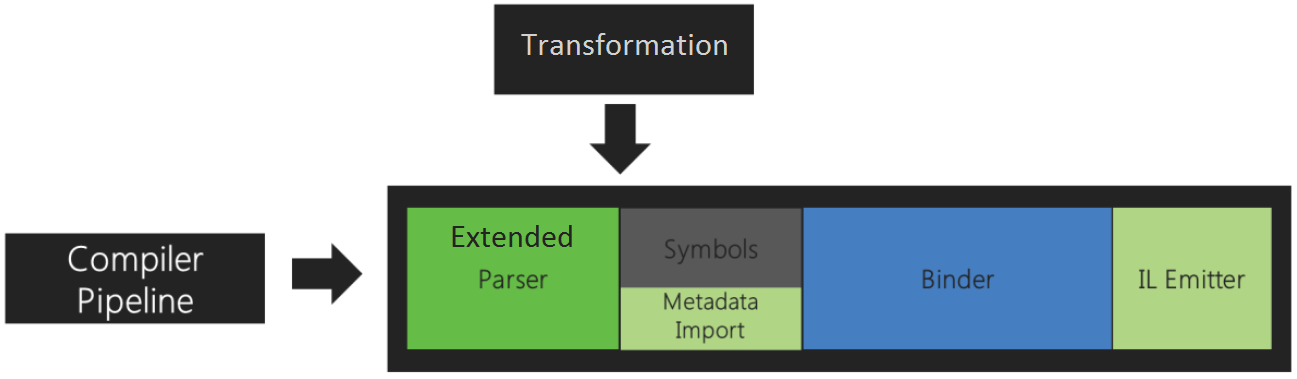
\includegraphics[width=1\textwidth]{\rootpath/worksheets/roslyn_extension/figures/compiler_pipeline_extension} 
 \caption{Extension occurs at the syntax tree and symbol level.}
\label{fig:compiler_pipeline_extension}
\end{figure}

The described approach was selected due to the following reasons:
\begin{enumerate}
\item As described in \bsref{subsec:roslyn_first_phase} the C\# lexer uses a simple \bscode{switch} case to identify tokens by choosing the type of token to identify based on the first character of the token, while the parser uses a recursive descent technique, both of which are implemented by hand. Such techniques have a low degree of complexity, as one method corresponds to parsing one non-terminal, compared to strategies such as \ac{LALR}\cite{nunes2003cps}. Thus modifying the lexer and parser is simpler than if more complex techniques had been employed.

\item The Roslyn compiler generates the nodes composing its syntax trees along with factory methods and a visitor pattern implementation based on the content of an \ac{XML} file. Therefore adding new nodes to represent the extended language constructs, such as the \bscode{atomic} block and \bscode{retry} statement, simply amounts to adding definitions for these nodes to the \ac{XML}, allowing the employed tool to generate source code for the new nodes. 

\item As described in \bsref{sec:syntax_trees} Roslyn's syntax trees are designed to be fast to modify by reusing underlying green nodes instead of creating complete copies\cite[p. 6]{ng2012roslyn}. This speaks for conducting transformation on the level of the syntax tree despite its immutable implementation.

\item The Roslyn project has been designed to allow programmers to utilize the information gathered during the compilation phases, by analyzing the syntax tree, the information in the symbol table and the results of semantics analysis. These parts of the compiler are exposed as a public \ac{API} allowing access to both syntactic and semantic information. Utilizing this \ac{API} during the transformation phases allows the transformation to draw on the existing semantic analysis to answer questions such as, what method is the target of a method invocation, without the need for implementing complex analysis.

\item By parsing an extended syntax tree and transforming it into a regular C\# syntax tree, the existing semantic analysis and code emission implementations can be utilized.
\end{enumerate}

Despite of the many advantages of the selected approach, a number of disadvantages also exists. The following disadvantages were identified:
\begin{enumerate}
	\item By modifying the syntax tree, the roundtripable property is lost, as the syntax tree no longer represents the original source code. Consequently, it is not possible to inform the programmer of the placement of errors in generated code. This requires our own code analysis, to give meaningful errors attached to the original source code. Ultimately, the ability to rely on the existing code analysis provided by the Roslyn compiler is lost. Alternatively, we could perform the transformation at a later compilation phase, e.g. modifying the bound tree in the binding phase or do changes before emitting code in the emit phase. This would preserve the roundtripable property, but also limit the reuse of the existing compiler. 
	
	\item As \bscode{atomic} fields, properties and local variables are translated into a corresponding \ac{STM} type, the types need to be known. As C\# allows the programmer to utilize type inference for local variables, the type can be unknown at this point of compilation, thus making it impossible to identify which type the local variables should be translated to. To remedy this, we must infer the type before translation. Roslyn offers the possibility to evaluate the type of an expression, which we use to infer the type of \bscode{atomic} local variables of no type. Consequently, we must perform some of the work, that the Roslyn compiler does at later stages of the compilation, reducing the reuse of the later compilation phases.
\end{enumerate}

\section{Lexing \& Parsing Phases}
This section describes the changes conducted in order to extend the lexing and parsing phases of the Roslyn C\# compiler to support the constructs described in \bsref{chap:stm_design}.
\label{sec:roslyn_lexer_parser_changes}

\subsection{Lexer Changes}
As described in \bsref{chap:stm_design}, \stmnamesp introduces three new keywords: \bscode{atomic,} \bscode{orelse} and \bscode{retry}. As a result the lexer component has been extended to identify these keyword as tokens of the correct kind. The C\# lexer initially lexes keyword tokens as if they were identifiers. If an identified token corresponds to a keyword, a keyword token with the correct kind is used instead. 

Allowing the lexer to identify the new keywords required adding their definition to the lookup methods of the \bscode{SyntaxKindFacts} class. This class defines the \bscode{GetKeywordKind} which the lexer uses to identify the keyword kind of an identifier, if the identifier represents a keyword. Additionally, the \bscode{SyntaxKindFacts} class defines the \bscode{GetText} method for determining the string representation of a keyword based on its kind. A definition of the new keywords was added to this class.

To allow a token to represent the new keywords, the \bscode{AtomicKeyword}, \bscode{OrelseKeyword} and \bscode{RetryKeyword} entries were added to the \bscode{SyntaxKind} enumeration. As described in \bsref{subsubsec:roslyn_kinds}, the \bscode{SyntaxKind} enumeration contains an entry for each type of node, token, or trivia in C\#. Whenever the lexer identifies an occurrence of one of the new keywords, the corresponding kind is  returned. For example an occurrence of the \bscode{atomic} keyword results in a token with the kind \bscode{AtomicKeyword} returned.

\subsection{Syntax Tree Extension}
The design described in \bsref{chap:stm_design} adds the \bscode{atomic}, \bscode{orelse} and \bscode{retry} constructs which the existing syntax tree cannot express. Therefore the syntax tree must be extended to support these language constructs. As described in \bsref{subsec:roslyn_syntax_tree_generation} nodes composing the syntax tree, along with factory methods and the visitor pattern implementation, are generated on the basis of an \ac{XML} file. Adding additional nodes to the syntax tree therefore amounts to defining them in the \ac{XML} notation, which has been done for the three previously mentioned constructs. \bsref{lst:roslyn_extension_tre_xml} shows the \ac{XML} code defining the \bscode{AtomicStatementSyntax} node which represents an \bscode{atomic} block in the syntax tree. Line 1 defines the name and base class of the node while line 2 defines its kind. The \bscode{AtomicStatement} kind has been added to the \bscode{SyntaxKind} enumeration as described previously. Line 3 defines a property on the node which holds the token representing the \bscode{AtomicKeyword} which starts the definition of the atomic blocks. The property has a constraint specifying the kind of the token, that can be associated with the property which is defined on line 4 as well as a comment given on lines 5-9. Line 11 defines a statement property which holds the block of statements associated with the defined \bscode{atomic} block. Line 18 defines a property containing a \bscode{SyntaxList} of \bscode{orelse} blocks associated with the \bscode{atomic} block. This relationship has been modeled after the relationship between a C\# \bscode{try} statement and its \bscode{catch} clauses, as both have a zero to many association. Finally lines 25-27 defines a comment for the \bscode{AtomicStatementSyntax}, while line 28-30 defines a comment for the factory method.

\begin{lstlisting}[label=lst:roslyn_extension_tre_xml,
  caption={AtomicStatement \ac{XML} definition},
  language=XML,  
  showspaces=false,
  showtabs=false,
  breaklines=true,
  showstringspaces=false,
  breakatwhitespace=true,
  escapechar=~,
  morekeywords={Name, Base, Type}]  % Start your code-block

  <Node Name="AtomicStatementSyntax" Base="StatementSyntax">
    <Kind Name="AtomicStatement"/>
    <Field Name="AtomicKeyword" Type="SyntaxToken">
      <Kind Name="AtomicKeyword"/>
      <PropertyComment>
        <summary>
          Gets a SyntaxToken that represents the atomic keyword.
        </summary>
      </PropertyComment>
    </Field>
    <Field Name="Statement" Type="StatementSyntax">
      <PropertyComment>
        <summary>
          Gets a StatementSyntax that represents the statement to be executed when the condition is true.
        </summary>
      </PropertyComment>
    </Field>
    <Field Name="Orelses" Type="SyntaxList&lt;OrelseSyntax&gt;">
      <PropertyComment>
        <summary>
          Gets a SyntaxList containing the orelse blocks associated with the atomic statement.
        </summary>
      </PropertyComment>
    </Field>
    <TypeComment>
      <summary>Represents an atomic block.</summary>
    </TypeComment>
    <FactoryComment>
      <summary>Creates an AtomicStatementSyntax node</summary>
    </FactoryComment>
  </Node>
\end{lstlisting}

Declaration of transactional local variables, fields and parameters does not require modifications to the syntax tree as the standard nodes for these constructs allow a collection of modifiers to be associated with the declaration. Any atomic modifiers are simply added to the collection along with any other modifiers. 


\subsection{Parser Changes}
As described in \bsref{subsec:roslyn_first_phase} the C\# parser uses a recursive descent strategy implemented by hand. As it is customary for recursive descent implementations, each construct has a method responsible for parsing that particular construct. For the new \bscode{atomic}, \bscode{orelse} and \bscode{retry} such a method has been added, while the methods for parsing local variables, fields, parameters and properties have been modified to allow for an atomic modifier, as well as generating error messages for any unsupported modifier combinations such as \bscode{atomic const} and \bscode{readonly const}. Errors are associated with the erroneous nodes as it is customary for the compiler. A later compilation phase generates error messages and cancels code emission if any errors were present.

\bsref{lst:parse_atomic_block} shows the \bscode{ParseAtomicBlock} method responsible for parsing an \bscode{atomic} block. Line \ref{line:ab_keyword} parses an \bscode{atomic} keyword returning a token representing the keyword. Line \ref{line:ab_block} parses the block of statements representing the transaction body. Lines \ref{line:ab_orelse_start} to line \ref{line:ab_orelse_end} parses any \bscode{orelse} blocks associated with the \bscode{atomic} statement, if any are present. Line \ref{line:ab_allocate} allocates a \bscode{SyntaxListBuilder}. The \bscode{Allocate} method reuses existing space if possible, in order to limit the overhead of allocation. Line \ref{line:ab_parse_orelse} delegates the parsing of the actual \bscode{orelse} block to its corresponding method. Line \ref{line:ab_free} frees the space allocated by the call on line \ref{line:ab_allocate}. The \bscode{try finally} construct ensures that the space is freed in case of an exception. Finally on line \ref{line:ab_return} the syntax factory is used to create the \bscode{AtomicStatementSyntax} that is returned.

\begin{lstlisting}[label=lst:parse_atomic_block,
  caption={Method for parsing \bscode{atomic} block},
  language=Java,  
  showspaces=false,
  showtabs=false,
  breaklines=true,
  showstringspaces=false,
  breakatwhitespace=true,
  commentstyle=\color{greencomments},
  keywordstyle=\color{bluekeywords},
  stringstyle=\color{redstrings},
  escapechar=~,
  morekeywords={atomic, retry, orElse, var, get, set}]  % Start your code-block

  private StatementSyntax ParseAtomicBlock()
  { 
    var atomicKeyword = this.EatToken(SyntaxKind.AtomicKeyword);~\label{line:ab_keyword}~
    var block = this.ParseEmbeddedStatement(false);~\label{line:ab_block}~

    var orelses = SyntaxFactory.List<OrelseSyntax>();~\label{line:ab_orelse_start}~
    var orelseBuilder = _pool.Allocate<OrelseSyntax>();~\label{line:ab_allocate}~
    try
    {
      while (this.CurrentToken.Kind == SyntaxKind.OrelseKeyword)
      {
        var clause = ParseOrelse();~\label{line:ab_parse_orelse}~
        orelseBuilder.Add(clause);
      }

      orelses = orelseBuilder.ToList();~\label{line:ab_tolist}~
    }
    finally
    {
      _pool.Free(orelseBuilder);~\label{line:ab_free}~
    }~\label{line:ab_orelse_end}~

    return _syntaxFactory.AtomicStatement(atomicKeyword, block, orelses);~\label{line:ab_return}~
  }
\end{lstlisting}
%error codes, const atomic, readonly atomic

\subsection{Symbol Changes}
The symbols representing fields, local variables, and parameters have been modified with a new \bscode{IsAtomic} property of type \bscode{bool}, indicating if they represent an atomic variation of these constructs. The logic which creates the symbol table has further been modified to, for each of these constructs, determine whether the declaration is atomic and set the \bscode{IsAtomic} to the appropriate value.

For each usage of a field, local variable or parameter, the semantic model allows for the retrieval of a symbol, representing the corresponding declaration. Based on the added \bscode{IsAtomic} property this symbol can be used to determine whether the usage represents the usage of an atomic variable. For cases where only access to atomic variables has be modified, the symbol extension allows easy access to the required information.

\section{Syntax Tree Transformations}
\label{sec:syntax_tree_transformations}
This section presents examples of the syntax tree transformations performed during the compilation process. In order to prevent errors due to ambiguity between type names, the transformation process uses fully qualified names\cite[p. 73]{csharp2013specificaiton}  for any types in the \ac{STM} library. In the examples presented in this section the simple names have been used, in order to improve readability. 

\subsection{Atomic Block}
In \bsref{subsec:design_atomic_block} the design for the \bscode{atomic} block is described. \bsref{lst:before_atomic_block} depicts the syntax of the atomic block before transformation. 

\begin{lstlisting}[label=lst:before_atomic_block,
  caption={\bscode{atomic} Block Before Transformation},
  language=Java,  
  showspaces=false,
  showtabs=false,
  breaklines=true,
  showstringspaces=false,
  breakatwhitespace=true,
  commentstyle=\color{greencomments},
  keywordstyle=\color{bluekeywords},
  stringstyle=\color{redstrings},
  morekeywords={atomic, retry, orelse, var, get, set}]  % Start your code-block

  atomic
  {
    //Block
  }
  orelse
  {
    //Orelse block
  }
\end{lstlisting}
The transformation of an atomic block is done over the following four steps:
\begin{enumerate}
	\item Construct a syntax node for a lambda expression (anonymous function) with a body equal to that of the atomic block.
	\item Construct lambda expressions for any \bscode{orelse} blocks associated with the \bscode{atomic} blocks, preserving their bodies as with the \bscode{atomic} block.
	\item Construct a syntax node for the invocation of the \bscode{STMSystem.Atomic} method, giving the created lambda expressions as arguments.
	\item Replace the \bscode{atomic} block with the invocation of the \bscode{STMSystem.Atomic} method.
\end{enumerate}
For syntax shown in \bsref{lst:before_atomic_block} the transformation produces the output shown in \bsref{lst:after_atomic_block}.

\begin{lstlisting}[label=lst:after_atomic_block,
  caption={\bscode{atomic} Block After Transformation},
  language=Java,  
  showspaces=false,
  showtabs=false,
  breaklines=true,
  showstringspaces=false,
  breakatwhitespace=true,
  commentstyle=\color{greencomments},
  keywordstyle=\color{bluekeywords},
  stringstyle=\color{redstrings},
  morekeywords={atomic, retry, orelse, var, get, set}]  % Start your code-block

  STMSystem.Atomic(() => {
    //Block					
  },
  () => {
    //Orelse block
  });
\end{lstlisting}
As a consequence of translating an atomic block into a lambda, return statements inside the lambda do not return out of the atomic block as described in \bsref{subsec:design_atomic_block}. In order to ensure the wanted semantics, an analysis is performed to identify all atomic blocks containing return statements. In such a case, a return statement is added before the method invocation. Return statements inside nested transactions must return out of the entire transaction. To accommodate this, the analysis also identifies nested transactions.

\subsection{Field Types}\label{subsec:extension_field}
In \bsref{subsec:design_trans_field} we described the design of transactional fields. Any field declared \bscode{atomic} must have its type substituted to the corresponding \ac{STM} type in order for the \ac{STM} system to track any changes to the variable. If a specialized type exist, such as \bscode{TMInt} for \bscode{int}, then that type is used. Otherwise the generic \bscode{TMVar} is used.  As the \ac{STM} types act as a wrapper object allowing the \ac{STM} system to track how the wrapped value is access, all atomic fields must be initialized to an instance of a \bscode{STM} type as accessing the wrapped value will otherwise cause a \bscode{NullReferenceException}. If an initializer expression is given as part of the field declaration the constructor of the wrapping \ac{STM} object is given the expression as an argument, initializing the wrapped value to the value computed by the initializer expression. If no initializer expression is given the wrapped value is initialized to the default value for the wrapped type by instantiating the \ac{STM} object using its parameterless constructor. The transformation of a atomic field declaration follows the steps described below:

\begin{enumerate}
	\item Determine the type of the wrapping \ac{STM} objects based on the type of the field declaration.
	\item For each variable declared as part of the field declaration, construct an object instantiation expression following the approach described above. This expression serves as the new initializer for the particular variable it was created for.
	\item Construct a new field declaration with the same access modifier and variable names as the original declaration, but substituting the type with the \ac{STM} object type and initializer expressions with the created object instantiation expressions.
	\item Replace the original field declaration with the newly the constructed field declaration. 
\end{enumerate}

\bsref{lst:before_atomic_field} presents a example of two \bscode{atomic} field declarations before transformation while \bsref{lst:after_atomic_field} shows the result of applying the transformation. Line \ref{line:af_field1_before} of \bsref{lst:before_atomic_field} is transformed to line \ref{line:af_field1_after} of \bsref{lst:after_atomic_field}. The type of the field is changed to the specialized integer \ac{STM} type \bscode{TMInt} and the initializer expression is used to initialized the value of the created \bscode{TMInt} object. Line \ref{line:af_field2_before} of \bsref{lst:before_atomic_field} is transformed to line \ref{line:af_field2_after} of \bsref{lst:after_atomic_field}. The type is transformed to \bscode{TMVar<string>}. For \bscode{field3}, which original definition does not contain an initializer expression, a initializer expression has been created following the previously described procedure.
 
\begin{lstlisting}[label=lst:before_atomic_field,
  caption={\bscode{atomic} Field Before Transformation},
  language=Java,  
  showspaces=false,
  showtabs=false,
  breaklines=true,
  showstringspaces=false,
  breakatwhitespace=true,
  escapechar=~,
  commentstyle=\color{greencomments},
  keywordstyle=\color{bluekeywords},
  stringstyle=\color{redstrings},
  morekeywords={atomic, retry, orelse, var, get, set}]  % Start your code-block

  public class AtomicFieldExample
  {
    private atomic int field1 = 1;~\label{line:af_field1_before}~
    public atomic string field2 = "Hello world!", field3;~\label{line:af_field2_before}~
  }
\end{lstlisting}

\begin{lstlisting}[label=lst:after_atomic_field,
  caption={\bscode{atomic} Field After Transformation},
  language=Java,  
  showspaces=false,
  showtabs=false,
  breaklines=true,
  showstringspaces=false,
  breakatwhitespace=true,
  escapechar=~,
  commentstyle=\color{greencomments},
  keywordstyle=\color{bluekeywords},
  stringstyle=\color{redstrings},
  morekeywords={atomic, retry, orelse, var, get, set, string}]  % Start your code-block

  public class AtomicFieldExample
  {
    private TMInt field1 = new TMInt (1);~\label{line:af_field1_after}~
    public TMVar<string> field2 = new TMVar<string>("Hello world!"), field3 = new TMVar<string>();~\label{line:af_field2_after}~
  }
\end{lstlisting}
 

\subsection{Properties}
In \bsref{subsec:design_properties} we described the design for transactional properties. In order to provide the wanted semantics, we transform it into two parts: an atomic backing field, and a manual property. The transformation takes the following approach for each transactional property identified in the syntax tree:

\begin{enumerate}
	\item Constructs a get-body with the access-modifier of the original property's get. The get-body contains a block in which a return to the backing field are. The backing field is not yet constructed, but a method is used to determine its future identifier to ensure a correct reference.
	\item Constructs a set-body with the access-modifier of the original property's set. The set-body contains a block in which an assignment of \bscode{value} is made to the backing field.
	\item Constructs a manual property with the access modifier of the original property, the get-body and set-body constructed earlier.
	\item Constructs a private transactional field of the same type as the original property, used as backing field.
\end{enumerate}
\andreas{The code performing the transformation can be found in: STM.cs - ReplaceProperties(SyntaxNode root)}

The transactional properties are transformed before the transactional fields, thus enabling reuse of the transformation done for atomic fields, as the backing field can be constructed as a transactional field instead of fully transforming it. Additionally, no transformation has to be done for the manual form, as the transactional field used for backing the property is processed as described in \bsref{subsec:extension_field}. The automatic form before translation is exemplified in \bsref{lst:before_atomic_property}:

\begin{lstlisting}[label=lst:before_atomic_property,
  caption={Before Transformation},
  language=Java,  
  showspaces=false,
  showtabs=false,
  breaklines=true,
  showstringspaces=false,
  breakatwhitespace=true,
  commentstyle=\color{greencomments},
  keywordstyle=\color{bluekeywords},
  stringstyle=\color{redstrings},
  morekeywords={atomic, retry, orElse, var, get, set, string}]  % Start your code-block

  class Car {
      public atomic int KmDriven { get; set; }
  }
\end{lstlisting}

The result of transforming the example in \bsref{lst:before_atomic_property} is shown in \bsref{after_atomic_property}.
\begin{lstlisting}[label=lst:after_atomic_property,
  caption={After Transformation},
  language=Java,  
  showspaces=false,
  showtabs=false,
  breaklines=true,
  showstringspaces=false,
  breakatwhitespace=true,
  commentstyle=\color{greencomments},
  keywordstyle=\color{bluekeywords},
  stringstyle=\color{redstrings},
  morekeywords={atomic, retry, orElse, var, get, set}]  % Start your code-block

  class Car {
    private atomic int _kmDriven;
    public int KmDriven {
        get {
            return _kmDriven;
        }
        set {
            _kmDriven = value;
            // Announce value changes
        }
    }
  }
\end{lstlisting}

\andreas[inline]{We dont protect against a naming conflict of the generated backing field and an existing field.}

\subsection{Local Variables}
In \bsref{subsec:local_variables} we described the wanted design for transactional local variables. 
Just like fields annotated with atomic, annotated local variables must have its type substituted to a corresponding \ac{STM} type. Thus, the approach is similar to the one described in \bsref{subsec:extension_field}, with the exception that a local variable can be declared without specifying the type by using the \bscode{var} keyword, relying on compile-time type inference to determine the type. Since the type is not determined at this point, we utilize Roslyn's \ac{API} to infer the type, and replace the \bscode{var} keyword with the type. This is done by identifying all local declaration statements with the type \bscode{var} and annotated \bscode{atomic}. The transformation is exemplified with an example of before on \bsref{lst:before_atomic_variable} on line \ref{line:av_variable1_before}, a local variable is declared by using the \bscode{var} keyword. The entire r-value of the statement is an expression, which can be evaluated to a type, by utilizing the Roslyn compiler \ac{API}. In \bsref{lst:after_atomic_variable} on line  \ref{line:av_variable1_after} the result shows that the type was infered to a \bscode{string}, thus the \bscode{var} is replace by a \bscode{TMVar<string>}.

\begin{lstlisting}[label=lst:before_atomic_variable,
  caption={\bscode{atomic} Local Variables Before Transformation},
  language=Java,  
  showspaces=false,
  showtabs=false,
  breaklines=true,
  showstringspaces=false,
  breakatwhitespace=true,
  escapechar=~,
  commentstyle=\color{greencomments},
  keywordstyle=\color{bluekeywords},
  stringstyle=\color{redstrings},
  morekeywords={atomic, retry, orelse, var, get, set}]  % Start your code-block

  public class AtomicVarExample
  {
    public void Method()
    {
      atomic var variable1 = "Hello World!";~\label{line:av_variable1_before}~
      atomic int variable2 = 42;~\label{line:av_variable2_before}~
    }
  }
\end{lstlisting}

\begin{lstlisting}[label=lst:after_atomic_variable,
  caption={\bscode{atomic} Local Variables After Transformation},
  language=Java,  
  showspaces=false,
  showtabs=false,
  breaklines=true,
  showstringspaces=false,
  breakatwhitespace=true,
  escapechar=~,
  commentstyle=\color{greencomments},
  keywordstyle=\color{bluekeywords},
  stringstyle=\color{redstrings},
  morekeywords={atomic, retry, orelse, var, get, set, string}]  % Start your code-block

  public class AtomicVarExample
  {
    public void Method()
    {
      TMVar<string> variable1 = new TMVar<string>("Hello World!");~\label{line:av_variable1_after}~
      TMInt variable2 = new TMInt(42);~\label{line:av_variable2_after}~
    }
  }
\end{lstlisting}

\subsection{Accessing Transactional Variables}
\label{subsec:roslyn_extension_accessing_variables}
As described in \bsref{subsec:stm_impl_transactional_variables} setting the value of a transactional variable is done through the \bscode{Value} property of the supplied \ac{STM} types. As the type of any field, local variable or property declared \bscode{atomic} in \stmnamesp is changed to the corresponding \ac{STM} type, any assignment must go through the \bscode{Value} property. As described in \bsref{subsec:stm_impl_transactional_variables} the \ac{STM} types supply support for implicit conversion to the wrapped value, when appearing as r-values. The transformation can however not rely on implicit conversion in all cases as, for example the comparison of two \bscode{TMInt} objects results in reference comparison instead of the expected integer comparison. As such, also the r-value appearances of any transactional field, local variable and parameter must be transformed to access the \bscode{Value} property ensuring that the wrapped object is accessed instead of the \ac{STM} object. Special handling is given to the \bscode{++} and \bscode{--} operators as the numeric \bscode{STM} types supply transactional implementations of these operators. The transformation ensures that these operators access the \ac{STM} object directly instead of access the \bscode{Value} property.

The implementations for the transformation of access to transactional variables are divided into two parts. The first dealing with the usage of a transactional variable occurring as a single identifier such as \bscode{someTMVar}. The second part handles member access expressions such as \bscode{object.tmfield1.tmfield2}. While these two implementations differ in the syntactic constructs they work on, their overall approach both follow the steps described below:

\begin{enumerate}
	\item Identify each usage of a transactional field, local variable, or parameter including both r- and l-value occurrences.
	\item Construct a member access expression accessing the \bscode{Value} property of the identified variable.
	\item Replace the usage of the variable with the constructed member access expression. 
\end{enumerate}

\bsref{lst:before_atomic_usage} presents an example accessing both a transactional field, local variable and parameter. \bsref{lst:after_atomic_usage} shows the result of applying the transformation to the example presented in \bsref{lst:before_atomic_usage}. The assignment on line \ref{line:au_assigment} of \bsref{lst:before_atomic_usage} is transformed to access the \bscode{Value} property of both its left and right sides, as both of the variable involved are transactional. The result of the transformation is shown on line \ref{line:au_assigment_after} of \bsref{lst:after_atomic_usage}. The member access expression on line \ref{line:au_member_access} of \bsref{lst:before_atomic_usage} is likewise transformed to access the \bscode{Value} property of both transactional fields involved. The resulting code is shown on line \ref{line:au_member_access_after} of \bsref{lst:after_atomic_usage}.

\begin{lstlisting}[label=lst:before_atomic_usage,
  caption={Usage of \bscode{atomic} Variables Before Transformation},
  language=Java,  
  showspaces=false,
  showtabs=false,
  breaklines=true,
  showstringspaces=false,
  breakatwhitespace=true,
  escapechar=~,
  commentstyle=\color{greencomments},
  keywordstyle=\color{bluekeywords},
  stringstyle=\color{redstrings},
  morekeywords={atomic, retry, orelse, var, get, set}]  % Start your code-block

  public class AtomicExample
  {
    public atomic AtomicExample aField;

    public AtomicExample ExampleMethod(atomic int i)
    {
      atomic int k = 0;
      k = i;~\label{line:au_assigment}~

      return aField.aField;~\label{line:au_member_access}~
    }
  }
\end{lstlisting}

\begin{lstlisting}[label=lst:after_atomic_usage,
  caption={Usage of \bscode{atomic} Variables After Transformation},
  language=Java,  
  showspaces=false,
  showtabs=false,
  breaklines=true,
  showstringspaces=false,
  breakatwhitespace=true,
  escapechar=~,
  commentstyle=\color{greencomments},
  keywordstyle=\color{bluekeywords},
  stringstyle=\color{redstrings},
  morekeywords={atomic, retry, orelse, var, get, set}]  % Start your code-block

  public class AtomicExample
  {
    public TMVar<AtomicExample> aField = new TMVar<AtomicExample>();

    public AtomicExample ExampleMethod(TMInt i)
    {
      TMInt k = new TMInt(0);
      k.Value = i.Value;~\label{line:au_assigment_after}~

      return aField.Value.aField.Value;~\label{line:au_member_access_after}~
    }
  }
\end{lstlisting}

\subsection{Parameters}
\label{subsec:roslyn_extension_parameters}
As with transactional local variables and transactional fields, the type of a parameter declared atomic must be changed to the corresponding \ac{STM} type in order for the \ac{STM} system to track assignments to it. \bsref{lst:before_atomic_parameter} presents a method taking two \bscode{atomic} parameters while \bsref{lst:after_atomic_parameter} presents the result of applying the parameter transformation. Each atomic parameter is transformed individually and any \bscode{ref} or \bscode{out} modifiers are preserved.

\begin{lstlisting}[label=lst:before_atomic_parameter,
  caption={\bscode{atomic} Parameters Before Transformation},
  language=Java,  
  showspaces=false,
  showtabs=false,
  breaklines=true,
  showstringspaces=false,
  breakatwhitespace=true,
  escapechar=~,
  commentstyle=\color{greencomments},
  keywordstyle=\color{bluekeywords},
  stringstyle=\color{redstrings},
  morekeywords={atomic, retry, orelse, var, get, set}]  % Start your code-block

  public class AtomicParameterExample
  {
    public void TestMethod(atomic int x, bool b, atomic ref string s)~\label{line:ap_before}~
    {
      //Body
    }
  }
\end{lstlisting}

\begin{lstlisting}[label=lst:after_atomic_parameter,
  caption={\bscode{atomic} Parameters After Transformation},
  language=Java,  
  showspaces=false,
  showtabs=false,
  breaklines=true,
  showstringspaces=false,
  breakatwhitespace=true,
  escapechar=~,
  commentstyle=\color{greencomments},
  keywordstyle=\color{bluekeywords},
  stringstyle=\color{redstrings},
  morekeywords={atomic, retry, orelse, var, get, set, ref}]  % Start your code-block

  public class AtomicParameterExample
  {
    public void TestMethod(TMInt x, bool b, ref TMVar<string> s)~\label{line:ap_after}~
    {
      //Body
    }
  }
\end{lstlisting}

\subsubsection{Transactional Output Parameters}
Transactional output parameters described in \bsref{subsec:stm_desgin_out_parameters} require additional handling as C\# requires every execution path in the method body to assign a value to the parameter\cite[p. 42]{sestoft2011c}. As described in \bsref{subsec:roslyn_extension_accessing_variables}, any assignment to the variable is replaced with an assignment to its \bscode{Value} property. As a consequence no assignments occur to the variable itself resulting in an error in the generated code. To rectify this error, an assignment, assigning a new \ac{STM} object with the same type as the parameter, is generated in the top method body for every \bscode{atomic out} parameter of that particular method. For each \bscode{atomic out} the \stmnamesp transformation contains the following steps:

\begin{enumerate}
	\item Construct an object initialization expression creating a new \ac{STM} object of the same type as the parameter.
	\item Construct a assignment statement assigning the newly constructed object initialization expression to the \bscode{atomic out} parameter.
	\item Insert the assignment statement as the first statement in the body of the enclosing method declaration.
\end{enumerate}

\bsref{lst:before_atomic_out_parameter} shows a method with an \bscode{atomic out} parameter while \bsref{lst:after_atomic_out_parameter} shows the result of applying the transformation.
Based on the \bscode{atomic out} parameter declared on line \ref{line:aout_before} of \bsref{lst:before_atomic_out_parameter} the assignment on line \ref{line:aout_after} of \bsref{lst:after_atomic_out_parameter} is generated.

\begin{lstlisting}[label=lst:before_atomic_out_parameter,
  caption={\bscode{atomic out} Parameter Before Transformation},
  language=Java,  
  showspaces=false,
  showtabs=false,
  breaklines=true,
  showstringspaces=false,
  breakatwhitespace=true,
  escapechar=~,
  commentstyle=\color{greencomments},
  keywordstyle=\color{bluekeywords},
  stringstyle=\color{redstrings},
  morekeywords={atomic, retry, orelse, var, get, set, ret, out}]  % Start your code-block

  public class AtomicOutExample
  {
    public static void TestMethodAtomic(atomic out int i, int j)~\label{line:aout_before}~
    {
      i = 12;
      j = 12;
    }
  }
\end{lstlisting}

\begin{lstlisting}[label=lst:after_atomic_out_parameter,
  caption={\bscode{atomic out} Parameter After Transformation},
  language=Java,  
  showspaces=false,
  showtabs=false,
  breaklines=true,
  showstringspaces=false,
  breakatwhitespace=true,
  escapechar=~,
  commentstyle=\color{greencomments},
  keywordstyle=\color{bluekeywords},
  stringstyle=\color{redstrings},
  morekeywords={atomic, retry, orelse, var, get, set, ret, out}]  % Start your code-block

  public class AtomicOutExample
  {
    public static void TestMethodAtomic(out TMInt i, int j)
    {
      i = new TMInt();~\label{line:aout_after}~
      i.Value = 12;
      j = 12;
    }
  }
\end{lstlisting}

While the generated assignment solves the problem of assignments to \bscode{atomic out} parameters being translated to a assignment to the \ac{STM} objects \bscode{Value} property, it introduces two new problems. Firstly, C\# requires that every \bscode{out} parameter is assigned a value before a method exists, generating a compile time error if that is not the case\cite[p. 94]{csharp2013specificaiton}. This error message is lost for transactional output parameters due to the generated assignment. Secondly, C\# requires that a out parameter is assigned to before reading from it\cite[p. 94]{csharp2013specificaiton}, generating a compile time error if a read occurs before a \bscode{out} parameter is assigned a value. If a read occurs before any assignment in the original source code, no error is given due to the generated assignment. In both cases an meaningful error can be generated by applying analysis to a transactional output parameters \bscode{Value} following the rules defined in\cite[p. 95]{csharp2013specificaiton}. No such analysis has however been implemented in the initial prototype of \stmname.


\subsection{Arguments}
As described in \bsref{subsec:stm_desgin_value_parameters} \stmnamesp support value parameters. Replacing the type of atomic parameters with the corresponding \ac{STM} type, as described in \bsref{subsec:roslyn_extension_parameters}, results in a type mismatch when calling a method with an \bscode{atomic} parameter of some type $T$ as the parameter is no longer of type $T$, but of $T$'s corresponding \ac{STM} type. As a result transformation must be applied to arguments passed to an \bscode{atomic} parameter, ensuring that the argument represents an object of the required \ac{STM} type. The transformation of an argument to an \bscode{atomic} parameter goes through the following steps:

\begin{enumerate}
	\item Determine the \ac{STM} type of the formal parameter to which the argument corresponds.
	\item Construct an object initialization expression creating an object of the previously determined \ac{STM} type, giving the argument expression as an argument to the constructor of the object.
	\item Replace the argument with the constructed object initialization expression.
\end{enumerate}

\bsref{lst:before_atomic_argument} presents an example of calling a method with an \bscode{atomic} parameter, while \bsref{lst:after_atomic_argument} shows the result of the transformation. Line \ref{line:aa_param_before} is transformed as described in \bsref{subsec:roslyn_extension_parameters}. Line \ref{line:aa_before} in \bsref{lst:before_atomic_argument} is transformed to line \ref{line:aa_after} in \bsref{lst:after_atomic_argument}. The argument to the \bscode{atomic} parameter is replaced with an object initialization expression creating a new \bscode{TMInt} object which is initialized using the original argument.

\begin{lstlisting}[label=lst:before_atomic_argument,
  caption={\bscode{atomic} Argument Before Transformation},
  language=Java,  
  showspaces=false,
  showtabs=false,
  breaklines=true,
  showstringspaces=false,
  breakatwhitespace=true,
  escapechar=~,
  commentstyle=\color{greencomments},
  keywordstyle=\color{bluekeywords},
  stringstyle=\color{redstrings},
  morekeywords={atomic, retry, orelse, var, get, set, ret, out}]  % Start your code-block

  public class AtomicArgumentExample
  {
    public static void TestMethod(atomic int x, int y)~\label{line:aa_param_before}~
    {
      //Body
    }

    public static void Main()
    {
      TestMethod(1, 2);~\label{line:aa_before}~
    }
  }
\end{lstlisting}

\begin{lstlisting}[label=lst:after_atomic_argument,
  caption={\bscode{atomic} Argument After Transformation},
  language=Java,  
  showspaces=false,
  showtabs=false,
  breaklines=true,
  showstringspaces=false,
  breakatwhitespace=true,
  escapechar=~,
  commentstyle=\color{greencomments},
  keywordstyle=\color{bluekeywords},
  stringstyle=\color{redstrings},
  morekeywords={atomic, retry, orelse, var, get, set, ret, out}]  % Start your code-block

  public class AtomicArgumentExample
  {
    public static void TestMethod(TMInt x, int y)
    {
      //Body
    }

    public static void Main()
    {
      TestMethod(new TMInt(1), 2);~\label{line:aa_after}~
    }
  }
\end{lstlisting}

\subsubsection{Ref/Out Arguments}
Supporting \bscode{atomic} \bscode{ref} and \bscode{out} parameters, as described in \bsref{subsubsec:trans_ref_out_args}, presents a problem due to the type mismatch as a result of transforming the parameters. \bscode{ref} and \bscode{out} parameters require the argument to be an assignable variable of the same type as the parameter. As the type of the parameter is transformed, a variable of type $T$ can not be passed directly as \bscode{ref} or \bscode{out} to an \bscode{atomic} parameter of type $T$.

Four different cases exist for passing \bscode{ref} and \bscode{out} parameters. These are:
\begin{enumerate}
	\item $T$ $\quad \rightarrow \quad$ \bscode{atomic} $T$
	\item \bscode{atomic} $T$ $\quad \rightarrow\quad$ $T$
	\item \bscode{atomic} $T$ $\quad \rightarrow\quad$ \bscode{atomic} $T$
	\item $T$ $\quad \rightarrow \quad$ $T$
\end{enumerate} 
where $T$ is some arbitrary type, $\text{ } \bscode{atomic} \quad  T$ is $T$'s corresponding \ac{STM} type and $\text{ } \bscode{atomic} \quad T \quad \rightarrow \quad T$ describes passing an argument of type $T$ into a parameter of the \ac{STM} type corresponding to $T$. The third and fourth cases are handled by the C\# compiler so transformation must only be applied in cases one and two.
For each argument node in the syntax tree the transformation goes through the following steps:
\begin{enumerate}
	\item Determine whether the argument represents one of the two previously described cases. If so, the remaining transformation steps are applied.
	\item Construct a syntax node for a local variable with a type definition equal to that of the parameter, initializing it using the original argument and insert it just before the method call
	\item Replace the original argument with an identifier equal to the name of the previously generated intermediate local variable passed using the same modifier as the original argument
	\item Construct an assignment syntax node assigning the value of the intermediate local variable to the original argument and insert it just after the method call
\end{enumerate}

\bsref{lst:before_atomic_ref} shows an example containing three method calls, where the first and third call falls in one of the categories which require transformation. Applying the transformation to the example presented in \bsref{lst:after_atomic_ref} produces a syntax tree representing the code shown in \bsref{lst:after_atomic_ref}. Line \ref{line:aref1} of \bsref{lst:before_atomic_ref} is transformed to lines \ref{line:aref1_after_1} to \ref{line:aref1_after_3} of \bsref{lst:after_atomic_ref}. As the parameter is \bscode{atomic} the local variable inserted on line \ref{line:aref1_after_1} is of the parameters corresponding \ac{STM} type. The argument to the method call has been replaced as seen on line \ref{line:aref1_after_2}. The assignment on line \ref{line:aref1_after_3} assigns the value computed by the called method to the original argument. Line \ref{line:aref2} of \bsref{lst:before_atomic_ref} is not transformed as it represents the case \bscode{atomic} $T$ $\quad \rightarrow \quad$ \bscode{atomic} $T$. Line \ref{line:aref3} of \bsref{lst:before_atomic_ref} is transformed much like \ref{line:aref1}, except the generated local field is of type \bscode{int} instead of a \ac{STM} type, as the parameter is not declared \bscode{atomic}. C\# requires the argument for a \bscode{ref} or \bscode{out} parameter to be a variable. For the case $T$ $\quad \rightarrow \quad$ \bscode{atomic} $T$ and \bscode{atomic} $T$ $\quad \rightarrow \quad$ $T$,  compile time analysis has been implemented to generate an error if the original argument does not correspond to a variable, as this would otherwise always be the case.

%In order simplify the language and maintain the same semantics whenever a atomic parameter or variable is passed as an argument or 

\begin{lstlisting}[label=lst:before_atomic_ref,
  caption={\bscode{ref} Arguments Before Transformation},
  language=Java,  
  showspaces=false,
  showtabs=false,
  breaklines=true,
  showstringspaces=false,
  breakatwhitespace=true,
  escapechar=~,
  commentstyle=\color{greencomments},
  keywordstyle=\color{bluekeywords},
  stringstyle=\color{redstrings},
  morekeywords={atomic, retry, orelse, var, get, set, ref, out}]  % Start your code-block

  public class AtomicRefExample
  {
    public static void TestMethodAtomic(atomic ref int i)
    {
      i = 12;
    }

    public static void TestMethod(ref int i)
    {
      i = 12;
    }

    public static void Main()
    {
      int i = 10;
      atomic int iAtomic = 10;

      TestMethodAtomic(ref i);~\label{line:aref1}~
      TestMethodAtomic(ref iAtomic);~\label{line:aref2}~
      TestMethod(ref iAtomic);~\label{line:aref3}~
    }
  }
\end{lstlisting}

\begin{lstlisting}[label=lst:after_atomic_ref,
  caption={\bscode{ref} Arguments After Transformation},
  language=Java,  
  showspaces=false,
  showtabs=false,
  breaklines=true,
  showstringspaces=false,
  breakatwhitespace=true,
  escapechar=~,
  commentstyle=\color{greencomments},
  keywordstyle=\color{bluekeywords},
  stringstyle=\color{redstrings},
  morekeywords={atomic, retry, orelse, var, get, set, ref, out}]  % Start your code-block

  public class AtomicRefExample
  {
    public static void TestMethodAtomic(ref TMInt i)
    {
      i.Value = 12;
    }

    public static void TestMethod(ref int i)
    {
      i = 12;
    }

    public static void Main()
    {
      int i = 10;
      TMInt iAtomic = new TMInt(10);

      TMInt _gen1 = new TMInt(i);~\label{line:aref1_after_1}~
      TestMethodAtomic(ref _gen1);~\label{line:aref1_after_2}~
      i = _gen1.Value;~\label{line:aref1_after_3}~

      TestMethodAtomic(ref iAtomic);~\label{line:aref2_after_1}~

      int _gen3 = iAtomic.Value;~\label{line:aref3_after_1}~
      TestMethod(ref _gen3);~\label{line:aref3_after_2}~
      iAtomic.Value = _gen3;~\label{line:aref3_after_3}~
    }
  }
\end{lstlisting}

\subsection{Retry}
In \bsref{sec:sync_design} the design of conditional synchronization through the use of \bscode{retry} is described. As \bscode{retry} is a keyword used as a statement, much like the \bscode{break} and \bscode{continue} statements in C\#, the transformation need to identify all \bscode{retry} keywords and replace them with a method invocation to the static method \bscode{STMSystem.Retry} defined in the \ac{STM} library, described in \bsref{subsec:impl_retry}. The library then carries out the effect of the \bscode{retry} statement. To inform programmers of unintended behavior, analysis generating a warning if the retry statement is used outside of an \bscode{atomic} or \bscode{orelse} block, has has been implemented. 

\section{Testing}
Testing is employed to ensure the Roslyn extension fulfills the design decisions of \stmnamesp and the integration with existing language features described in \bsref{chap:stm_design}.

For the reasons described in \bsref{sec:stm_impl_testing}, unit testing is chosen for testing the Roslyn extension. Unit testing is valuable in relation to the maintenance and further development of the Roslyn extension. Furthermore, Roslyn is still under heavy development, which means radical changes will happen. The unit test suite is beneficial to test if the extension still works, whenever new changes are made to Roslyn. The disadvantage of unit testing being more time consuming than ad hoc testing is outweighed by the many advantages which is gained. Additionally, each unit test is built using a black-box testing strategy\cite[p. 87]{graham2008foundations}, where the program is viewed as a black box and focus is only on the input and output. This is done as the focus of the unit tests is on the functionality of the compiler. That is, the tests focus on what it does, and not on how it does it. Additionally it fits well with how a compiler is normally treated, as it is treated as a black-box where the input and output is only available.\toby{er grunden til black-box fin nok?}

Each \ac{STM} construct and each integration with an existing language feature is covered by at least a single unit test. Furthermore, integration with disallowed existing language features is tested, e.g. there is a unit test that ensures an error is produced if the programmer tries to declare a method with an atomic optional parameter. This results in a rather extensive test suite, which is valuable in relation to the correctness of the \ac{STM} constructs and integration with language features of \stmname.\toby{Er sidste sætning fin nok?}

In \bsref{lst:empty_atomic_block} is shown an example of a unit test for an empty atomic block. On line \ref{line:ab_finalstr} the string \bscode{finalStr} to be compiled is generated using the bscode{MakeSkeletonWithMain} method, which generates a test namespace, class and main method, with the supplied string arguments \bscode{strInClass} and \bscode{strInMain} included. Afterwards the string is written to a test file, which is used as argument in the method on line \ref{line:ab_runcsc}, which executes \bscode{csc.exe} (C\# command line compiler) and returns a \bscode{CmdRes} object that contains the command line output. On line \ref{line:ab_assertcsc} it is checked that the command line output does not contain any warning, error or invalid exitcode. For unit tests that check error generations, f.x. an illegal existing language featured is used with an \ac{STM} construct, this step is not present, instead \bscode{CmdRed} can be checked if it contains the expected error or warning. On line \ref{line:ab_expecstr} the expected result of compilation string \bscode{expecStr} is generated and on line \ref{line:ab_compiledstr} the actual compilation string \bscode{compiledStr} is fetched. In order to retrieve the actual compilation string, csc.exe is extended with an additional argument called \bscode{stmiout}, which writes the source code after \ac{STM} transformation to the specified path. This argument is used in the method on line \ref{line:ab_runcsc}. Finally on line \ref{line:ab_asserteq} the expected string and the actually compiled string is checked for equality, if equal the test passes and otherwise it fails. Before checking for equality, the \bscode{AssertEqualStrings} method removes formatting from the strings.

\begin{lstlisting}[label=lst:empty_atomic_block,
  caption={Empty Atomic Block Unit Test},
  language=Java,  
  showspaces=false,
  showtabs=false,
  breaklines=true,
  showstringspaces=false,
  breakatwhitespace=true,
  escapechar=~,
  commentstyle=\color{greencomments},
  keywordstyle=\color{bluekeywords},
  stringstyle=\color{redstrings},
  morekeywords={atomic, retry, orelse, var, get, set, ref, out, Test}]  % Start your code-block
  [Test]
  public void AtomicBlockEmpty()
  {
  		string finalStr = MakeSkeletonWithMain(~\label{line:ab_finalstr}~
  			strInClass: "",
  			strInMain: "atomic{\n\t\t\t"+ 
  				"}");
  		StringToTestFile(finalStr);~\label{line:ab_strtofile}~
  		CmdRes res = RunCscWithOutAndStmIOut();~\label{line:ab_runcsc}~
  		AssertCmdRes(res);~\label{line:ab_assertcsc}~
  		
  		string expecStr = MakeSkeletonWithMain(~\label{line:ab_expecstr}~
  			strInClass: "",
  			strInMain: STM.STMNameSpace + ".STMSystem.Atomic(" +
  				"() =>" +
  				"{" +
  				"});");
			string compiledStr =~\label{line:ab_compiledstr}~ TestFileToString(currentCompiledCsFile);
			AssertEqualStrings(expecStr, compiledStr);~\label{line:ab_asserteq}~
  }
\end{lstlisting}

\toby[i]{Hvad med errors? Errorcode og stm diagnostics bag?}
%ERRORS: (hvordan smides de) - er det her det skal besrkives?
	%STM diagnostic for semantic errors
	%errors i paraser, kan bruge ErrorCode Enum osv.

\section{Design \& Integration Revisited}
This section describes areas in which the initial prototype implementation described in this chapter, conflicts with the intended design and language integration described in \bsref{chap:stm_design}. Ideally no conflicts would happen, as the analysis in the design and language integration chapter would foresee them. However, implementing the design gave an insight and knowledge into unforeseen areas.

\subsection{Transactional Local Variables and Fields}
As described in \bsref{subsec:extension_field} and \bsref{subsec:local_variables} local variables and fields of type $T$ declared \bscode{atomic} are transformed to declarations with a type equal to $T$'s corresponding \ac{STM} type. As part of this process the local variable or field is initialized to \ac{STM} object of the correct type, using any initializer expression if present. If not, the default value of the variable is initialized to the default value of type $T$ through the \ac{STM} object's parameter less constructor. 

For fields this presents no issue as fields are always initialized to the default value of their type if no initializer expression is present\cite[p. 93]{csharp2013specificaiton}. This is however not the case for local variables. The C\# compiler generates an error if a local variable is accessed before it has been assigned a value\cite[p. 96]{csharp2013specificaiton}. As \bscode{atomic} local variables are always initialized, this error will never occur for such variables, which can lead to unintended behavior in cases where the programmer forgets to assign an \bscode{atomic} local variable. In such cases the default value of the \bscode{atomic} local variables original type will be the value accessed, potentially leading to some confusion.

In order to provide similar error messages for \bscode{atomic} local variables as for regular C\# local variables, the flow analysis detecting whether a given local variable has been assigned a value when it is accessed, must be extended to track both initial assignment as part of the declaration, as well as assignment to \bscode{STM} objects \bscode{Value} as opposed to assignments directly to the variable. Such analysis has however not been included in the initial prototype described in this chapter.\lone{Why not?}

\subsection{Transactional Optional Parameters}
C\# requires that the default value given when declaring an optional parameter is one of the following\cite[p. 309]{csharp2013specificaiton}:
\begin{enumerate}
	\item A constant expression
	\item An expression of the form \bscode{new S()} where \bscode{S} is a value type
	\item An expression of the form \bscode{default(S)} where \bscode{S} is a value type
\end{enumerate}
As described in \bsref{subsec:roslyn_extension_parameters} the transformation of an \bscode{atomic} parameter transforms the type of the parameter to one of the \ac{STM} types. Providing a default value to an \bscode{atomic} parameter therefore amounts to initializing a new \ac{STM} object with the same type as the parameter supplying the defined default value to its constructor. All \ac{STM} types are however reference types and the creation of a new \ac{STM} object can therefore, per the three rules described above, not be supplied as the replacement default value as this would result in a compile time error. As such default values for transactional value parameters are not implemented in the initial prototype described in this chapter. Analysis has been implemented to produce an error if an \bscode{atomic} value parameter is given a default value. This is done in the parsing phase, by checking if a parameter is declared with the \bscode{atomic} modifier and has an optional value.


\subsection{Transactional Ref/Out Parameters \& Arguments}
As described in \bsref{subsec:stm_desgin_ref_parameters} and \bsref{subsec:stm_desgin_out_parameters} the intended design was that assignment to transactional \bscode{ref/out} parameters takes effect when the transaction in which the assignment takes place, commits. This behavior holds true for the case:
\begin{itemize}
	\item $\bscode{atomic} \quad T \quad \rightarrow \quad \bscode{atomic} \quad T$
\end{itemize}
That is, the case involving an \bscode{atomic} argument and parameter. For the cases:
\begin{itemize}
	\item $T \quad \rightarrow \quad \bscode{atomic} \quad T$
	\item $\bscode{atomic} \quad T \quad \rightarrow \quad T$
\end{itemize}
the behavior is however different. Due to the type mismatch between the argument and parameter, an intermediate local variable is passed as the actual argument, and the original argument is assigned as the first thing after the call finishes. This conflicts with traditional C\#, where any assignment to a \bscode{ref/out} parameter takes effect immediately\cite[p. 76]{sestoft2011c}. If the parameter is declared \bscode{atomic} and the method call is wrapped in an \bscode{atomic} block, there will be no difference in timing as any assignments to atomic variables take effect when the transaction commits. However, if the call is not wrapped in a atomic block the difference in timing can have unintended consequences, especially when considering concurrent execution. Due to this issue a number of ways for handling \bscode{atomic ref/out} parameters and arguments were investigated:
\begin{enumerate}
	\item Warning the programmer if one of the two problematic cases is used
	\item Disallowing the two problematic cases described above
	\item Disallowing \bscode{atomic ref/out} parameters
\end{enumerate}
In C\#, passing a volatile field as \bscode{ref/out} results in the field being treated as non volatile within the method body\cite{csharpVolatileRef}. If such an operation is detected the compiler creates a warning informing the programmer of the change in semantics. The same approach could be taken whenever one of the two problematic cases described earlier is detected.

Disallowing \bscode{atomic ref/out} parameters, preventing the programmer from declaring \bscode{atomic ref/out} parameters, removes the timing issues present in the cases where an intermediate \bscode{atomic} variable is required. However, the ability to pass an \bscode{atomic} variable by reference is lost and the case of passing a variable of type \bscode{atomic} $T$ into a parameter of type $T$ is still unsolved. Consequently, this would limit the orthogonality of the \bscode{atomic} construct.

Disallowing \bscode{ref/out} the cases where both an \bscode{atomic} and non \bscode{atomic} variable/parameter are involved removes the cases where the desired timing cannot be provided. However, it will, for example, no longer be possible to pass an \bscode{atomic} integer into an \bscode{out} integer parameter such as that of \bscode{Int32.TryParse.} Such restrictions limits the flexibility when using \bscode{atomic} variables, and the programmer needs to circumvent this,  by the use of intermediate variables which clutters the intention of the code, and reduces the readability.

For the initial prototype presented in this chapter the first option of warning the programmer of the change in semantics has been selected. This ensures that the change in semantics is not hidden from the programmer thereby allowing her to adapt the program. \andreas{Write something about the approach done in c\# with volatile fields passed into methods}.The impact of the feature will be closely observed throughout the evaluation with the aim of determining the final form of the feature, or even if the feature should be part of the language at all.\andreas{We MUST follow up on this in the evaluation}

\toby[i]{Fejl med variable \bscode{i} ikke er initialiseret, hvis man prøver at returnere \bscode{i}, hvor \bscode{i} bliver assigned i en indre nested atomic.}

\worksheetend